%% abtex2-modelo-trabalho-academico.tex, v-1.9.7 laurocesar
%% Copyright 2012-2018 by abnTeX2 group at http://www.abntex.net.br/
%%
%% This work may be distributed and/or modified under the
%% conditions of the LaTeX Project Public License, either version 1.3
%% of this license or (at your option) any later version.
%% The latest version of this license is in
%%   http://www.latex-project.org/lppl.txt
%% and version 1.3 or later is part of all distributions of LaTeX
%% version 2005/12/01 or later.
%%
%% This work has the LPPL maintenance status `maintained'.
%%
%% The Current Maintainer of this work is the abnTeX2 team, led
%% by Lauro César Araujo. Further information are available on
%% http://www.abntex.net.br/
%%
%% This work consists of the files abntex2-modelo-trabalho-academico.tex,
%% abntex2-modelo-include-comandos and abntex2-modelo-references.bib
%%

% ------------------------------------------------------------------------
% ------------------------------------------------------------------------
% abnTeX2: Modelo de Trabalho Academico (tese de doutorado, dissertacao de
% mestrado e trabalhos monograficos em geral) em conformidade com
% ABNT NBR 14724:2011: Informacao e documentacao - Trabalhos academicos -
% Apresentacao
% ------------------------------------------------------------------------
% ------------------------------------------------------------------------

\documentclass[
	% -- opções da classe memoir --
	12pt,				% tamanho da fonte
	openright,
	twoside,
	a4paper,			% tamanho do papel.
	% -- opções da classe abntex2 --
	% -- opções do pacote babel --
	brazil,			% idioma adicional para hifenização
	french,				% idioma adicional para hifenização
	spanish,			% idioma adicional para hifenização
	english				% o último idioma é o principal do documento
	]{abntex2}

\usepackage[T1]{fontenc}
\usepackage[utf8]{inputenc}
\usepackage{indentfirst}
\usepackage{color}
\usepackage{graphicx}
\usepackage{microtype}
\usepackage{amsmath}
\usepackage{amssymb}
\usepackage{ltablex}
\usepackage{subcaption}
\usepackage{pgfplots}
\pgfplotsset{width=10cm,compat=1.9}
\usepgfplotslibrary{external}
\usepgfplotslibrary{statistics}
\tikzexternalize
\usetikzlibrary{arrows.meta}
\usetikzlibrary{decorations.text}
\usepackage{hhline}
\usepackage{array}
\usepackage{colortbl}
\usepackage{multirow}
\usepackage{placeins}
\usepackage{makecell}
\usepackage[brazilian,hyperpageref]{backref}
\usepackage[alf]{abntex2cite}

\makeatletter
\@addtoreset{chapter}{part}
\makeatother

\renewcommand{\backrefpagesname}{Cited in page(s):~}
\renewcommand{\backref}{}
\renewcommand*{\backrefalt}[4]{
	\ifcase #1 %
		No citation in text.%
	\or
		Cited in page #2.%
	\else
		Cited #1 times in pages #2.%
	\fi}%

\newcommand{\oo}{\textordmasculine\ }

\newcommand{\tablemonofirst}[5]{%
	\renewcommand{\ArgX}{#1}
	\renewcommand{\ArgXI}{#2}
	\renewcommand{\ArgXII}{#3}
	\renewcommand{\ArgXIII}{#4}
	\renewcommand{\ArgXIV}{#5}
}

\newcommand{\tablemonosecond}[9]{%
	\begin{table}[h]
		\centering
		\caption{Analysis of solutions of #1 in water}
		\label{#2}
		\bgroup
		\def\arraystretch{1.5}
		\scalebox{0.9}{%
		\begin{tabular}{| p{0.2\textwidth} | p{0.4\textwidth} | %
				p{0.4\textwidth} |}\hline
			\multirow{2}*{Composition} &
				\multicolumn{2}{c|}{Models}\\\hhline{~--}
			& Raoult & Virial\\\hhline{-~~}
			\multirow{5}*{\makecell[l]{Water,\\#1}} &
				$\frac{\sqrt{\sum\text{deviations}^2}}{n}=#3$ &
				$\frac{\sqrt{\sum\text{deviations}^2}}{n}=#4$%
					\\\hhline{~-~}
			& UNIQUAC & $b_\text{#1}=#9$\\\hhline{~~-}
			& $\frac{\sqrt{\sum\text{deviations}^2}}{n}=#5$ & Norrish\\
			& $q_\text{water}=\ArgXI$ &
				$\frac{\sqrt{\sum\text{deviations}^2}}{n}=#6$\\
			& $q_\text{#1}=\ArgXIII$ & $K_\text{#1}=\ArgX$%
				\\\hhline{-~~}
			$\bar{a_w}=#7$ & $u_\text{water}=\ArgXII$ & \\
			$\bar{x_w}=#8$ & $u_\text{#1}=\ArgXIV$ & \\\hline
		\end{tabular}}
		\egroup
	\end{table}
}

\newcommand{\tablebifirstzero}[9]{%
	\newcommand{\ArgX}{#1}
	\newcommand{\ArgXI}{#2}
	\newcommand{\ArgXII}{#3}
	\newcommand{\ArgXIII}{#4}
	\newcommand{\ArgXIV}{#5}
	\newcommand{\ArgXV}{#6}
	\newcommand{\ArgXVI}{#7}
	\newcommand{\ArgXVII}{#8}
	\newcommand{\ArgXVIII}{#9}
}
\newcommand{\tablebifirst}[9]{%
	\renewcommand{\ArgX}{#1}
	\renewcommand{\ArgXI}{#2}
	\renewcommand{\ArgXII}{#3}
	\renewcommand{\ArgXIII}{#4}
	\renewcommand{\ArgXIV}{#5}
	\renewcommand{\ArgXV}{#6}
	\renewcommand{\ArgXVI}{#7}
	\renewcommand{\ArgXVII}{#8}
	\renewcommand{\ArgXVIII}{#9}
}
\newcommand{\tabletrisecondzero}[9]{%
	\newcommand{\ArgXIX}{#1}
	\newcommand{\ArgXX}{#2}
	\newcommand{\ArgXXI}{#3}
	\newcommand{\ArgXXII}{#4}
	\newcommand{\ArgXXIII}{#5}
	\newcommand{\ArgXXIV}{#6}
	\newcommand{\ArgXXV}{#7}
	\newcommand{\ArgXXVI}{#8}
	\newcommand{\ArgXXVII}{#9}
}
\newcommand{\tablebisecond}[2]{%
	\renewcommand{\ArgXIX}{#1}
	\renewcommand{\ArgXX}{#2}
}

\newcommand{\tablebithird}[9]{%
	\begin{table}[h]
		\centering
		\caption{Analysis of solutions of #1 and #2 in water}
		\label{#3}
		\bgroup
		\def\arraystretch{1.5}
		\scalebox{0.9}{%
		\begin{tabular}{| p{0.2\textwidth} | p{0.4\textwidth} | %
				p{0.4\textwidth} |}\hline
			\multirow{2}*{Composition} &
				\multicolumn{2}{c|}{Models}\\\hhline{~--}
			& Raoult & Virial\\\hhline{-~~}
			\multirow{7}*{\makecell[l]{Water,\\#1 and\\#2}} &
				$\frac{\sqrt{\sum\text{deviations}^2}}{n}=#9$ &
				$\frac{\sqrt{\sum\text{deviations}^2}}{n}=#7$%
					\\\hhline{~-~}
			& UNIQUAC & $b_\text{#1}=\ArgX$\\
			& $\frac{\sqrt{\sum\text{deviations}^2}}{n}=#8$ &
				$b_\text{#2}=\ArgXI$\\
			& $q_\text{water}=\ArgXV$ &
				$c_\text{#1/#2}=\ArgXII$\\\hhline{~~-}
			& $q_\text{#1}=\ArgXVII$ & Norrish \\
			& $q_\text{#2}=\ArgXIX$ &
				$\frac{\sqrt{\sum\text{deviations}^2}}{n}=#6$ \\
			& $u_\text{water}=\ArgXVI$ & $K_\text{#1}=\ArgXIII$%
				\\\hhline{-~~}
			$\bar{a_w}=#4$ & $u_\text{#1}=\ArgXVIII$ &
				$K_\text{#2} = \ArgXIV$ \\
			$\bar{x_w}=#5$ & $u_\text{#2}=\ArgXX$ & \\\hline
		\end{tabular}}
		\egroup
	\end{table}
}

\newcommand{\tabletrifirst}[9]{%
	\renewcommand{\ArgX}{#1}
	\renewcommand{\ArgXI}{#2}
	\renewcommand{\ArgXII}{#3}
	\renewcommand{\ArgXIII}{#4}
	\renewcommand{\ArgXIV}{#5}
	\renewcommand{\ArgXV}{#6}
	\renewcommand{\ArgXVI}{#7}
	\renewcommand{\ArgXVII}{#8}
	\renewcommand{\ArgXVIII}{#9}
}

\newcommand{\tabletrisecond}[9]{%
	\renewcommand{\ArgXIX}{#1}
	\renewcommand{\ArgXX}{#2}
	\renewcommand{\ArgXXI}{#3}
	\renewcommand{\ArgXXII}{#4}
	\renewcommand{\ArgXXIII}{#5}
	\renewcommand{\ArgXXIV}{#6}
	\renewcommand{\ArgXXV}{#7}
	\renewcommand{\ArgXXVI}{#8}
	\renewcommand{\ArgXXVII}{#9}
}

\newcommand{\tabletrithird}[9]{%
	\begin{table}[h]
		\centering
		\caption{Analysis of solutions of #1, #2 and \ArgXXVII\ in water}
		\label{#3}
		\bgroup
		\def\arraystretch{1.5}
		\scalebox{0.9}{%
		\begin{tabular}{| p{0.2\textwidth} | p{0.4\textwidth} | %
				p{0.4\textwidth} |}\hline
			\multirow{2}*{Composition} &
				\multicolumn{2}{c|}{Models}\\\hhline{~--}
			& Raoult & Virial\\\hhline{-~~}
			\multirow{10}*{\makecell[l]{Water,\\#1,\\#2 and\\\ArgXXVII}} &
				$\frac{\sqrt{\sum\text{deviations}^2}}{n}=#9$ &
				$\frac{\sqrt{\sum\text{deviations}^2}}{n}=#7$%
					\\\hhline{~-~}
			& UNIQUAC & $b_\text{#1}=\ArgX$\\
			& $\frac{\sqrt{\sum\text{deviations}^2}}{n}=#8$ &
				$b_\text{#2}=\ArgXI$\\
			& $q_\text{water}=\ArgXIX$ &
				$b_\text{\ArgXXVII} = \ArgXIII$ \\
			& $q_\text{#1}=\ArgXXI$ &
				$c_\text{#2/#1}=\ArgXII$\\
			& $q_\text{#2}=\ArgXXIII$
				& $c_\text{\ArgXXVII/#1}=\ArgXIV$\\
			& $q_\text{\ArgXXVII}=\ArgXXV$
				& $c_\text{\ArgXXVII/#2}=\ArgXV$\\\hhline{~~-}
			& $u_\text{water}=\ArgXX$ & Norrish \\
			& $u_\text{#1}=\ArgXXII$ &
				$\frac{\sqrt{\sum\text{deviations}^2}}{n}=#6$ \\
			& $u_\text{#2}=\ArgXXIV$ & $K_\text{#1}=\ArgXVI$%
				\\\hhline{-~~}
			$\bar{a_w}=#4$ & $u_\text{\ArgXXVII}=\ArgXXVI$ &
				$K_\text{#2} = \ArgXVII$ \\
			$\bar{x_w}=#5$ & & $K_\text{\ArgXXVII}=\ArgXVIII$ \\\hline
		\end{tabular}}
		\egroup
	\end{table}
}

\tablebifirstzero{1}{1}{1}{1}{1}{1}{1}{1}{1}
\tabletrisecondzero{1}{1}{1}{1}{1}{1}{1}{1}{1}

\newcolumntype{C}{>{\centering\arraybackslash}p{3em}}
\newcolumntype{R}{>{\raggedleft\arraybackslash}X}
\newcolumntype{G}{>{\columncolor{lightgray}\centering\arraybackslash}p{3em}}

\DeclareMathOperator*{\minimize}{minimize}

\titulo{Final Report for Undergraduate Research Project\\
	Thermodynamical Modelling of Solutions of Interest for the %
	Food Industry}
\autor{Pedro Henrique Callil Soares}
\local{São Paulo}
\data{2021}
\orientador{Pedro de Alcântara Pessoa Filho}
\instituicao{%
	Universidade de São Paulo -- USP
	\par
	Escola Politécnica
	\par
	Departamento de Engenharia Química}
\tipotrabalho{Undergraduate Research Project Report}
\preambulo{Undergraduate Research Project Report
	- analysis and modelling of water activity in solutions of carbohydrates
	and aminoacids.}



\definecolor{blue}{RGB}{41,5,195}
\definecolor{pverydarkblue}{rgb}{0,0,0.2}
\definecolor{pdarkblue}{rgb}{0,0,0.4}
\definecolor{pblue}{rgb}{0,0,0.6}
\definecolor{pbrightblue}{rgb}{0,0,0.8}
\definecolor{pverybrightblue}{rgb}{0,0,1.0}
\definecolor{pverydarkred}{rgb}{0.15,0,0}
\definecolor{pdarkred}{rgb}{0.3,0,0}
\definecolor{pred}{rgb}{0.45,0,0}
\definecolor{pbrightred}{rgb}{0.6,0,0}
\definecolor{pverybrightred}{rgb}{0.75,0,0}
\definecolor{pviolindarkred}{rgb}{0.7,0.5,0.5}
\definecolor{pviolinred}{rgb}{0.8,0.5,0.5}
\definecolor{pviolinbrightred}{rgb}{0.9,0.5,0.5}
\definecolor{pviolindarkblue}{rgb}{0.5,0.5,0.7}
\definecolor{pviolinblue}{rgb}{0.5,0.5,0.8}
\definecolor{pviolinbrightblue}{rgb}{0.5,0.5,0.9}
\definecolor{pbackground}{rgb}{0.9,0.9,0.87}
\definecolor{pplanned}{rgb}{0.8,0.8,0.8}
\definecolor{pdoing}{rgb}{0.65,0.65,0.8}
\definecolor{pdone}{rgb}{0.5,0.5,0.8}


\makeatletter
\hypersetup{
		pdftitle={\@title},
		pdfauthor={\@author},
		pdfsubject={\imprimirpreambulo},
		pdfcreator={LuaLaTeX},
		pdfkeywords={water activity} {carbohydrates} {aminoacids},
		colorlinks=true,
		linkcolor=blue,
		citecolor=blue,
		filecolor=magenta,
		urlcolor=blue,
		bookmarksdepth=4
}
\makeatother

\makeatletter
\setlength{\@fptop}{5pt}
\makeatother

%\newcommand{\quadroname}{Quadro}
%\newcommand{\listofquadrosname}{Lista de quadros}

%\newfloat[chapter]{quadro}{loq}{\quadroname}
%\newlistof{listofquadros}{loq}{\listofquadrosname}
%\newlistentry{quadro}{loq}{0}

%\setfloatadjustment{quadro}{\centering}
%\counterwithout{quadro}{chapter}
%\renewcommand{\cftquadroname}{\quadroname\space}
%\renewcommand*{\cftquadroaftersnum}{\hfill--\hfill}

%\setfloatlocations{quadro}{hbtp}


\setlength{\parindent}{1.3cm}

\setlength{\parskip}{0.2cm}

\makeindex

\begin{document}

\selectlanguage{english}

\frenchspacing

\imprimircapa

\imprimirfolhaderosto


\setlength{\absparsep}{18pt}
\begin{resumo}
	This project aims to build a database of water activity data in
	carbohydrate and aminoacid solutions, analysing the correlative
	capabilities of a number of models found in the literature. Water
	activity data as a function of composition were obtained from previous
	studies on the subject, and computational routines were programmed
	to evaluate the deviations between calculated osmotic coefficients
	(using models obtained through nonlinear least-squares fitting) and
	experimental data. Afterwards we performed an analysis of the influence
	of several factors in the correlative capabilities of each model.\\
	\textbf{Keywords}: carbohydrate solutions.
			aminoacid solutions.
			thermodynamical properties of solutions.
			water activity.
			thermodynamical modelling.
\end{resumo}

\pdfbookmark[0]{\listfigurename}{lof}
\listoffigures*
\cleardoublepage


\pdfbookmark[0]{\listtablename}{lot}
\listoftables*
\cleardoublepage

\begin{simbolos}
	\item[$ \gamma $] activity coefficient
	\item[$ \phi $] osmotic coefficient
	\item[$ \Pi $] osmotic pressure
	\item[$ a $] activity
	\item[$ C_p $] specific heat
	\item[$ f $] fugacity
	\item[$ \Delta H^\text{fus} $] enthalpy of vaporization
	\item[$ \Delta H^\text{vap} $] enthalpy of fusion
	\item[$ m $] molality
	\item[$ p^\text{vap} $] vapor pressure
	\item[$ X_i $] mass fraction (substance $i$)
	\item[$ x_i $] molar fraction (substance $i$)
	\item[$ \Xi_B, \Xi_F $] property $\Xi$ (boiling/freezing point)
	\item[$ \Xi^\text{ID} $] property $\Xi$ (ideal system)
	\item[$ \Xi^\text{ref} $] property $\Xi$ (reference system)
	\item[$ \Xi_w $] property $\Xi$ (water, \textit{e.g.} $a_w, %
		\gamma_w$, \textit{etc.} %
		for $\Xi = \alpha, \gamma$, \textit{etc.})
	\item[$K_i$] parameters for Norrish's model.
	\item[$b_i$, $c_{ij}$] parameters for virial model
	\item[$q_i$, $u_{ii}$] parameters for UNIQUAC model
	\item[$A_i$] parameters for a generic model
	\item[$\Phi$] osmotic coefficient estimate obtained through a generic model
\end{simbolos}

\pdfbookmark[0]{\contentsname}{toc}
\tableofcontents*
\cleardoublepage

\textual

\part{Introduction}

The activity $a$ of a substance in a system, defined \cite{sandler2017} as
the ratio between the fugacity of the substance in the system and its fugacity
in a reference system (equation \ref{eq:def_atv}), acts as its thermodynamically
``effective concentration''. Therefore, the measurement and analysis of the water
activity in solutions allows better predictions of phenomena related to the water
contents of a system. To the food industry, the most important of those phenomena
is the microbial-induced food spoilage.

Indeed, the property controlling microbial growth in a food product is the
water activity. In the graph exhibited at the figure
\ref{fig:germ}\footnote{\cite{canovas2007}}, one can see the values of water
activity required for the growth of a few microorganisms of interest.

\begin{figure}[h]
	\centering
	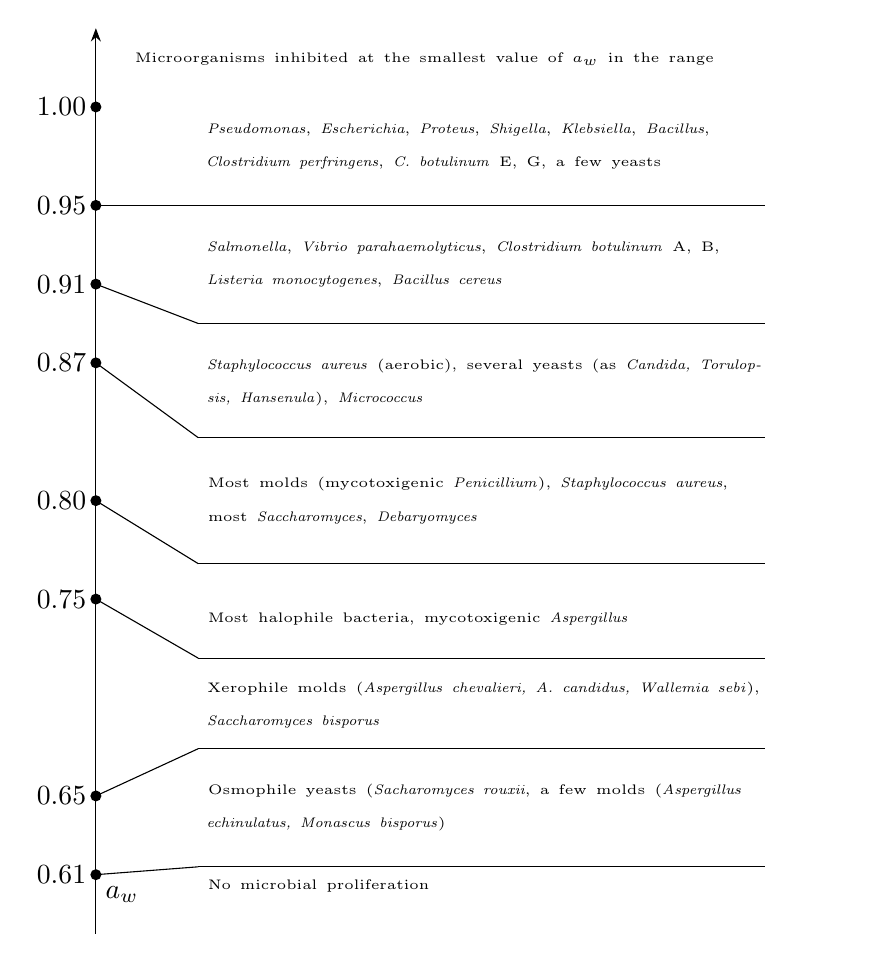
\begin{tikzpicture}[>=Stealth]
		\draw[->] (5,-0.5) -- (5,11);
		\draw (5,0.0) node[anchor=west] {$a_w$};
		\draw (5,8.75) -- (6.3,8.75);
		\draw (6.3,8.75) -- (13.5,8.75);
		\draw (5,7.75) -- (6.3,7.25);
		\draw (6.3,7.25) -- (13.5,7.25);
		\draw (5,6.75) -- (6.3,5.8);
		\draw (6.3,5.8) -- (13.5,5.8);
		\draw (5,5) -- (6.3,4.2);
		\draw (6.3,4.2) -- (13.5,4.2);
		\draw (5,3.75) -- (6.3,3);
		\draw (6.3,3) -- (13.5,3);
		\draw (5,1.25) -- (6.3,1.85);
		\draw (6.3,1.85) -- (13.5,1.85);
		\draw (5,0.25) -- (6.3,0.35);
		\draw (6.3,0.35) -- (13.5,0.35);
		\fill[black] (5,0.25) circle (0.07);
		\fill[black] (5,1.25) circle (0.07);
		\fill[black] (5,3.75) circle (0.07);
		\fill[black] (5,5) circle (0.07);
		\fill[black] (5,6.75) circle (0.07);
		\fill[black] (5,7.75) circle (0.07);
		\fill[black] (5,8.75) circle (0.07);
		\fill[black] (5,10) circle (0.07);
		\draw (10,10.4) node[anchor=south, text width=9cm]
		{\tiny{Microorganisms inhibited at the smallest value of
		$a_w$ in the range}};
		\draw (6.3,9.5) node[anchor=west, text width=7cm]
		{\tiny{\textit{Pseudomonas}, \textit{Escherichia},
		\textit{Proteus}, \textit{Shigella}, \textit{Klebsiella},
		\textit{Bacillus}, \textit{Clostridium perfringens},
		\textit{C. botulinum} E, G, a few yeasts}};
		\draw (6.3,8) node[anchor=west, text width=7cm]
		{\tiny{\textit{Salmonella}, \textit{Vibrio parahaemolyticus},
		\textit{Clostridium botulinum} A, B, \textit{Listeria
		monocytogenes}, \textit{Bacillus cereus}}};
		\draw (6.3,6.5) node[anchor=west, text width=7cm]
		{\tiny{\textit{Staphylococcus aureus} (aerobic), several
		yeasts (as \textit{Candida, Torulopsis, Hansenula}),
		\textit{Micrococcus}}};
		\draw (6.3,5) node[anchor=west, text width=7cm]
		{\tiny{Most molds (mycotoxigenic \textit{Penicillium}),
		\textit{Staphylococcus aureus},
		most \textit{Saccharomyces}, \textit{Debaryomyces}}};
		\draw (6.3,3.5) node[anchor=west, text width=7cm]
		{\tiny{Most halophile bacteria,
		mycotoxigenic \textit{Aspergillus}}};
		\draw (6.3,2.4) node[anchor=west, text width=7cm]
		{\tiny{Xerophile molds (\textit{Aspergillus chevalieri, A.
		candidus, Wallemia sebi}), \textit{Saccharomyces bisporus}}};
		\draw (6.3,1.1) node[anchor=west, text width=7cm]
		{\tiny{Osmophile yeasts (\textit{Sacharomyces rouxii},
		a few molds (\textit{Aspergillus echinulatus, Monascus
		bisporus})}};
		\draw (6.3,0.1) node[anchor=west, text width=7cm]
		{\tiny{No microbial proliferation}};
		\draw (5,0.25) node[anchor=east] {0.61};
		\draw (5,1.25) node[anchor=east] {0.65};
		\draw (5,3.75) node[anchor=east] {0.75};
		\draw (5,5) node[anchor=east] {0.80};
		\draw (5,6.75) node[anchor=east] {0.87};
		\draw (5,7.75) node[anchor=east] {0.91};
		\draw (5,8.75) node[anchor=east] {0.95};
		\draw (5,10) node[anchor=east] {1.00};
	\end{tikzpicture}
	\caption{$a_w$ values for microbial growth}
	\label{fig:germ}
\end{figure}

In the conditions usually found in the food industry, is reasonable to assume
that the gas phase of the system behaves as an ideal gas\cite{canovas2007},
in most situations. Furthermore, the reference condition is taken as pure and liquid
water at the same pressure and temperature as the system. Therefore, one can obtain:

\begin{equation}
	\label{eq:def_atv}
	a_w \equiv \left(\cfrac{f_w}{f^\text{ref}_w}\right)_T%
		\approx \left(\cfrac{p^\text{vap}_w}{p^\text{vap,ref}_w}\right)_T
\end{equation}

For ideal solutions, the evaluation of water activity is straightforward: for all
component $u$ in a mixture, its activity $a_i$ is simply its molar fraction $x_i$;
hence, $a_w = x_w$. However, not all systems are ideal, and therefore one needs to
adopt another property, the activity coefficient of the water, $\gamma_w$:

\begin{equation}
	a_w = \gamma_wx_w \implies \gamma_w = \cfrac{a_w}{x_w}
\end{equation}

Yet, even if one now has an indicator of the deviation of a solution from
ideality , another problem arises: the activity coefficient is not a good
parameter to evaluate the deviations when applied to very diluted solutions;
after all, $a_w=a_w(x_w)$ is a continuous function, and as the solution is diluted,
$a_w$ must go to 1 (because the limit $x_w=1$ is the reference solution), and
therefore one will observe that:

\begin{equation}
	\lim_{x_w \to 1}\gamma_w = 1
\end{equation}

And for many solutions of interest, one can observe not only high deviations from
ideal behavior, but also extremely diluted solutions. Thus, one adopts another
property, the osmotic coefficient $\phi$, defined as:

\begin{equation}
	\phi = \cfrac{\ln(a_w)}{\ln(x_w)}
\end{equation}

One can compare these two properties and visualize a possible behavior of
the water activity as the composition of a mixture changes by observing
the data plotted in the figure \ref{fig_atv_gamma_gluc} \cite{ebrahimi2016}.

\begin{figure}[h]
	\centering
	\begin{tikzpicture}
		\newsavebox{\minigrafglic}
		\savebox{\minigrafglic}{%
		\scalebox{0.5}{%
		\begin{tikzpicture}
			\begin{axis}[
			xmin=0.97,xmax=1.0,
			ymin=0.97,ymax=1.0,
			x dir=reverse,
			width=7cm,
			height=7cm,
			xlabel = {$x_w$},
			ylabel = {$a_w$},
			]
			\addplot+[
				color=pverydarkred,
				mark=o,
				only marks,
			]
			table[x={xw},y={aw}]{glucose_a_w_and_phi.dat};
			\addlegendentry{$a_w$ (experimental)};
			\addplot+[
				color=black,
				no marks,
				domain=0.96:1.0,
				samples=5,
			]{x};
			\addlegendentry{$a_w=x_w$};
		\end{axis}
	\end{tikzpicture}
	}}
	\begin{axis}[
			xmin = 0.97, xmax = 1.0, xlabel = {$x_w$},
			ymin = 0.96, ymax = 1.05, ylabel = {$\phi$},
			x tick label style={
				/pgf/number format/.cd,
				fixed,
				fixed zerofill,
				precision=3,
				/tikz/.cd
			},
			y tick label style={
				/pgf/number format/.cd,
				fixed,
				fixed zerofill,
				precision=3,
				/tikz/.cd
			},
			legend pos = south west,
			axis y line=left,
			x axis line style={-},
			xlabel near ticks,
			ylabel near ticks,
			x dir=reverse,
			ytick={0.97,0.985,1.00,1.015,1.03,1.045},
		]
		\addplot+[
			color=pdarkblue,
			mark=square,
			very thick,
			only marks,
		]
		table[x={xw},y={phi}]{glucose_a_w_and_phi.dat};
		\addlegendentry{$\phi$};
		\draw (axis cs: 0.981,0.99)node{\usebox{\minigrafglic}};
		\end{axis}
		\begin{axis}[
			xmin = 0.97, xmax = 1.0, xlabel = {$x_w$},
			ymin = 0.9977, ymax = 1.0001, ylabel = {$\gamma_w$},
			y tick label style={
				/pgf/number format/.cd,
				fixed,
				fixed zerofill,
				precision=4,
				/tikz/.cd
			},
			axis y line=right,
			axis x line=none,
			legend pos = south east,
			x dir=reverse,
		]
		\addplot+[
			color=pverybrightred,
			mark=o,
			very thick,
			only marks,
		]
		table[x={xw},y={gammaw}]{glucose_a_w_and_phi.dat};
		\addlegendentry{$\gamma_w$};
		\end{axis}
	\end{tikzpicture}
	\caption{Activity ($a_w$), Activity coefficient ($\gamma_w$) and%
	osmotic coefficient ($\phi$) of water in D-glucose solutions. %
	One should observe the difference in the $\gamma_w$ and $\phi$ axis scales.}
	\label{fig_atv_gamma_gluc}
\end{figure}

In addition, one must remember that water activity measurements are sometimes
obtained indirectly; instead of measurements of vapor pressure in the system
and comparison with the same property in the reference system (as shown in the
equation \ref{eq:def_atv}), one can measure properties as freezing point
depression, boiling point elevation, or the composition of another solution
in osmotic equilibrium with the system under analysis.

For instance, a few data sets obtained for $n$-ary solutions of carbohydrates
\cite{abderafi1994} are, in fact, boiling point elevation data. Hence, the
experimental measurements must first be converted to osmotic coefficient data,
through the equations \ref{eq:eleb_to_osco} \cite{ge2009,ge2009err}, which are
plotted in the figure \ref{fig_ge_and_wang}.

\begin{equation}
	\label{eq:eleb_to_osco}
	\begin{cases}
		\ln(a_w) = -\cfrac{\Delta H^\text{vap}_{0,T_B}\left(\cfrac{1}{T_B}%
			-\cfrac{1}{T_B+\Delta T_B}\right)-%
			\Delta C_p^\text{vap}\Bigg[\ln\left(\cfrac{T_B+%
			\Delta T_B}{T_B}\right) - \cfrac{\Delta T_B}{T_B+%
			\Delta T_B}\Bigg]}{R}\\
		\ln(a_w) = \cfrac{\Delta H^\text{fus}_{0,T_F}\left(\cfrac{1}{T_F}-%
		\cfrac{1}{T_F-\Delta T_F}\right)+\Delta C_p^\text{fus}%
		\Bigg[\ln\left(\cfrac{T_F-\Delta T_F}{T_F}\right) -%
		\cfrac{\Delta T_F}{T_F-\Delta T_F}\Bigg]}{R}
	\end{cases}
\end{equation}

\begin{figure}[h]
	\centering
	\begin{subfigure}{0.5\textwidth}
		\begin{tikzpicture}[scale=0.75]
			\begin{axis}[
				ylabel={$a_w$},
				xlabel={$T_B$[\textcelsius]},
				ymax=1, xmax=115, xmin=100,
			]
				\addplot [
					color=pred,
					no marks,
					very thick,
				]
					table [x={BPE},y={aw},col sep=comma]
						{ge_and_wang_bpe.csv};
			\end{axis}
		\end{tikzpicture}
		\caption{Boiling Point}
	\end{subfigure}%
	\hfill%
	\begin{subfigure}{0.5\textwidth}
		\begin{tikzpicture}[scale=0.75]
			\begin{axis}[
				ylabel={$a_w$},
				xlabel={$T_F$[\textcelsius]},
				ymax=1, xmin=-15, xmax=0,
			]
				\addplot [
					color=pblue,
					no marks,
					very thick,
				]
					table [x={FPD},y={aw},col sep=comma]
						{ge_and_wang_fpd.csv};
			\end{axis}
		\end{tikzpicture}
		\caption{Freezing Point}
	\end{subfigure}
	\caption{Relation between $T_B$/$T_F$ (in \textcelsius) and $a_w$, %
		$P=P_\text{atm}$}
	\label{fig_ge_and_wang}
\end{figure}


With $\Delta C_p$ defined as the difference in specific heat between the
phases: $\Delta C_p^\text{vap} = C_p^\text{vapor} -%
C_p^\text{liquid}$ and $\Delta C_p^\text{fus} = C_p^\text{liquid} -%
C_p^\text{solid}$, $\Delta T_F$ defined as the freezing point depression,
$\Delta T_B$ the boiling point elevation and $\Delta H_{0,T_B}^\text{vap}$ and
$\Delta H_{0,T_F}^\text{fus}$ representing the enthalpies of vaporization and fusion
of the solvent at $T_B$/$T_F$.

\part{Bibliographic Revision}

\chapter{Water activity modelling}

\section{Analysed models}

Several models were analysed, ranging in complexity from simple as Raoult's Law
or Caurie's equation to complex as the iterative procedure derived from the
Zdanovskii's relation or the UNIQUAC model, for subsequent comparison with a
virial equation (as in \ref{eq:ad_pessoa}, adapted from \cite{pessoa2008}, in
which $b_i$ and $c_{ij}$ are adjustable parameters and $\theta$ is a measure
of concentration).

\begin{equation}
	\label{eq:ad_pessoa}
	\ln(a_w) = \sum_{i \neq w}\theta_i\Bigg(1 +%
	2b_i+3\sum_{j \neq w}c_{ij}\theta_j\Bigg)
\end{equation}

For obtaining $a_w$ values in binary solutions, one has several distinct models
to choose from. From those models, the following shall be analysed and compared:

\begin{itemize}
	\item Raoult's Law: Simplest model, for ideal solutions. Assumes
		water activity $a_w = x_w$, its molar fraction;
	\item Norrish's Equation \cite{norrish1966}: Raoult's Law, corrected.
		One can, with the molar fraction of water, $x_w$, molar
		fraction of the other substance, $x_s$, and one adjustable
		parameter ($K$), utilize the equation \ref{eq_norrish} to
		obtain the water activity of a solution.
		\ref{eq_norrish}:
		\begin{equation}
			\label{eq_norrish}
			a_w = x_w\exp\Big[\Big(\sqrt{K}x_s\Big)^2\Big]
		\end{equation}
	\item UNIQUAC (\textit{universal quasi-chemical}) Model
		\cite{abrams1975}: Possibly the most complex model among the
		chosen ones; requiring two adjustable parameters for each pair
		of substances present in the mixture (between solvents and
		solutes), can be used for binary or $n$-ary systems. Even though
		the nonlinear fitting for the model presents a high computational
		cost, as we are dealing with simple mixtures (with a maximum of
		four components), the complexity of the model is not a problem.
\end{itemize}

For $n$-ary solutions, a few other models were chosen for analysis and
comparisons:

\begin{itemize}
	\item Raoult's Law: water activity $a_w$ equals $x_w$,
		its molar fraction;
	\item Norrish's Equation: adopted with a small modification to the equation
		\ref{eq_norrish}, as shown in the equation \ref{eq_norrish_multi};
		\begin{equation}
			\label{eq_norrish_multi}
			a_w = x_w\exp\Big[\Big(\sum_{i \neq w}%
			\sqrt{K_i}x_i\Big)^2\Big]
		\end{equation}
	\item Caurie's Model \cite{caurie1986}: water activity as a correction
		of the product of the water activities of binary solutions
		in which each component's molalities are either zero or equal
		to the its molality in the solution of interest, as presented
		in the equation \ref{eq_caurie}, in which $a_{wi}$ is the
		water activity in a binary solution in which the molality $m_i$
		of the substance $i$ remains the same and $n$ is the total number
		of solutes in the mixture.
		\begin{equation}
			\label{eq_caurie}
			a_w = \prod_{i \neq w}a_{wi}-\left[\cfrac{n}%
			{55.5^2}\sum_{\substack{i \neq j \\ i,j \neq w}}%
			m_im_j + \cfrac{(n+1)}{55.5^3}\sum_{%
			\substack{i\neq j,k \\ j \neq k \\  i,j,k \neq w}}%
			m_im_jm_k\right]
		\end{equation}
		To obtain the water activities of the binary solutions,
		we assumed ideal solution (Raoult's Law).
	\item Zdanovskii's Relation \cite{chen1973,sangster1973}:
		applied for ternary mixtures only, it's an iterative process
		based in the Zdanovskii relation; for a ternary mixture with
		two generic solutes 1 and 2, we adopt two binary solutions, one
		with 1 as its only solute, the other with 2, in osmotic equilibrium
		with the solution of interest. With $m_{01}$ and $m_{02}$ as the
		molalities of each solute in each the binary solution, and
		$m_1$ and $m_2$ as the molalities of each solute in the solution
		of interest, the Zdanovskii's relation ($m_1m_{01}^{-1} +
		m_2m_{02}^{-1} = 1$) generates an iterative procedure that
		returns the water activity of a ternary mixture from the
		curves $a_w=a_w(x_w)$ of binary mixtures of each solute.
	\item UNIQUAC (\textit{universal quasi-chemical}) Model, previously
		cited.
\end{itemize}

\section{Applicability of the models to the samples}

Since one is not only interested in fitting curves to data sets, but also in
assessing the possibility of predicting water activities for $n$-ary systems
based on data from binary systems, one can split the available models in two
great groups. For a thermodynamical model (as shown in equation
\ref{eq:geral_bigphi}) with $N$ parameters $(A_j)_{j \in \{1, 2, \ldots N\}}$
for the osmotic coefficient in a system of composition given by the molar
fractions of each component $(x_i)_\text{$i$ component}$, at temperature $T$
and pressure $P$, one can obtain estimates $(A^*_j)_{j \in \{1, 2, \ldots N\}}$
for the parameters through the use of nonlinear least-squares fitting,
as shown in equation \ref{eq:min_quad}, for a set of $K > N$ experimental data
points
$\{(\phi^k, T^k, P^k, (x_i)^k_\text{$i$ component}), k \in \{1,2,\ldots,K\}\}$.

\begin{equation}
	\label{eq:geral_bigphi}
	\phi = \Phi((A_j)_{j \in \{1, 2, \ldots, N\}}, (x_i)_\text{$i$ %
		component of the mixture}, T, P)
\end{equation}

\begin{equation}
	\label{eq:min_quad}
	\minimize_{(A_j^*)_{j \in \{1,2,\ldots,N\}} \in \mathbb{R}^N}%
	\left(\sum_{k \in \{1,2,\ldots,K\}}\left[\phi^k - \Phi((A^*_j)_{j%
	\in \{1, 2, \ldots, N\}}, (x^k_i)_\text{$i$ component},%
	T^k, P^k)\right]^2\right)
\end{equation}

For data obtained exclusively from binary systems, one may write:

\begin{equation}
	\forall k \in \{1,2,\ldots,K\} \;\; \exists i \neq w%
	\text{ component } : \forall \;\; i' \neq i, i' \neq w\;\; x^k_{i'} = 0
\end{equation}

When for all sets of data obtained exclusively from binary systems the equation
\ref{eq:no_bin_fit} is valid, one can say that the model presents an adjustable
parameter of component-component interaction. Otherwise, one can say that the model
has no parameters accounting for the interaction between two components.

\begin{equation}
	\label{eq:no_bin_fit}
	\exists j' \in \{1,2,\ldots,N\} : \forall \alpha \in \mathbb{R}\;\;%
	(A_j^*)_{j \in \{1,2,\ldots,N\}, A_{j'}^* = \alpha}%
	\text{ is a solution of \ref{eq:min_quad}}
\end{equation}

One must differentiate these two groups, for one of the aims of the project
is the assessment of the applicability of parameter estimates, obtained through
fitting curves through binary data, to $n$-ary data; this is important, primarily
because experimental data for binary systems are more abundant and easier to
obtain, but also due to the high computational cost in multivariate nonlinear
fitting.

An example of a model in the second category is the one proposed by Norrish; also,
one could trivially place models such as Zdanovskii's procedure and Caurie's
relation in the category. For the first one, more complex, the virial model defined
in the equation \ref{eq:ad_pessoa} or the UNIQUAC model can be considered as
examples.

\section{Limitations of the models and problems found}

One of the main problems found is the simple non-applicability of some models
to a few sets of data; as an example, one may check the intrinsical limitations
of the Norrish's model.

Norrish's model, as seen in the equations \ref{eq_norrish} and
\ref{eq_norrish_multi}, can be algebraically manipulated to yield equation
\ref{eq_phi_norrish} for the calculation of the osmotic coefficient $\phi$.

\begin{equation}
	\label{eq_phi_norrish}
	\phi = \cfrac{\ln(a_w)}{\ln(x_w)} = \cfrac{\ln(x_w) + \left(\sum_{ i\neq w}
	\sqrt{K_i}x_1\right)^2}{\ln(x_w)}
\end{equation}

As $x_w \le 1 \implies \ln(x_w) \le 0$, one can observe that the model can't
predict a value for $\phi$ greater than 1; however, this is not verified
in all real solutions, that can show several behaviors, ranging from
monotonically decreasing functions (as the model requires,\footnote{%
	Since $\lim_{x_w \to 1}\phi_\text{Norrish} = 1$.
} to monotonically increasing functions, the opposite of the desired
behavior, which can be seen in figure \ref{fig_atv_gamma_gluc}
and, more clearly, in figure \ref{fig_manose_phi}.

Another example is Caurie's equation; since $\lim_{x_w \to 0}m_i = +\infty$,
one can observe the existence of crtical dilutions, beyond which the
model simply fails to return a physically meaningful result, because
$a_w \in [0,1]$ and, as shown in the equations \ref{eq_caurie_fail},
there are values for the molar fractions of each component in the mixture
that, according to the model, must force the system to exhibit negative
values of $a_{w,\text{Caurie}}$. Besides, as the molar fraction of water
in a mixture decreases, $\phi$ must, in the limit, be as close as
desired to 0.

\begin{equation}
	\label{eq_caurie_fail}
	\begin{split}
		a_{w,\text{Caurie}} = \prod_{i \neq w}a_{w,i} - \left[\cfrac{n}%
			{55.5^2}\sum_{\substack{i \neq j \\ i,j \neq w}}%
			m_im_j + \cfrac{(n+1)}{55.5^3}\sum_{%
			\substack{i\neq j,k \\ j \neq k \\  i,j,k \neq w}}
			m_im_jm_k\right] <\\
		1 - \cfrac{n}{55.5^3}\left[55.5 \times%
			\sum_{\substack{i \neq j \\ i,j \neq w}}%
			m_im_j + \cfrac{n+1}{n}\sum_{%
			\substack{i\neq j,k \\ j \neq k \\  i,j,k \neq w}}
			m_im_jm_k\right]\implies\\
		\lim_{\substack{m_k \to +\infty \\%
				\forall n \neq k, \text{ $m_n$ constant}}}%
			a_{w,\text{Caurie}} = -\infty \implies%
		\lim_{x_w \to 0} a_{w,\text{Caurie}} = -\infty
	\end{split}
\end{equation}

This diversity of behaviors can be useful. For instance, for the virial model,
the measure chosen for the concentration was molar concentration, since one can
show that the data rarely follow the curves to which they are restricted when
one utilizes instead the molar fraction, as one would naïvely do. This can be
seen in the equations \ref{eq_phi_virial_mono_frac}
\footnote{%
	This can be affirmed since, $\forall w > 0$:
	\begin{equation*}
		\begin{split}
			e^w = 1 + w + \cfrac{w^2}{2!} + \ldots \ge w +1
			\stackrel{(z = w+1)}{\implies} e^z \ge ze \implies
				z \ge \ln(z) + 1
			\stackrel{\left(y=\cfrac{1}{z}\right)}{\implies}
				\cfrac{1}{y} \ge
				\ln\left(\cfrac{1}{y}\right) + 1 \implies\\
			1-y \ge y\ln\left(\cfrac{1}{y}\right)
			\stackrel{(x=1-y)}{\implies} x >
				(1-x)\ln\left(\cfrac{1}{1-x}\right)\implies
			\cfrac{x}{1-x} + \ln(1-x) > 0 \implies\\
				\cfrac{d}{dx}\left(\cfrac{x}{\ln(1-x)}\right) > 0
		\end{split}
	\end{equation*}
}
for binary systems, with $x$ as the molar fraction of the solute: the model
(with $\theta_i = x_i$) is obligatorily a monotonic function.

\begin{equation}
	\label{eq_phi_virial_mono_frac}
	\begin{split}
		\ln(a_w) = -x + 2bx \implies \phi =
			\cfrac{-x + 2bx}{\ln(1-x)}\implies\\
		\phi = (2b-1)\cfrac{x}{\ln(1-x)} \implies
			\forall (x_1,x_2) \in (0,1)\times(0,1)\;\;
			\cfrac{d\phi}{dx}\Big|_{x_1} \times
			\cfrac{d\phi}{dx}\Big|_{x_2} \ge 0
	\end{split}
\end{equation}

Another challenge (not intrinsical to the models, but specific to the data)
is the distribution of the data in small sets, compared to the amount of
data points required to fit a large model (as the complete UNIQUAC model,
for instance). Indeed, for a mixture of $n$ components, the model requires
$2n+n^2 \in \mathcal{O}(n^2)$ parameters (accounting for the interaction
energies $U_{ij}$ and the parameters $r_i$ and $q_i$. To solve this problem,
a few simplifications, from the literature, were adopted, as exhibited in
the equations \ref{eq_uniquac_simpl}.

\begin{equation}
	\label{eq_uniquac_simpl}
	\begin{cases}
		u_{ij} = \sqrt{u_{ii}u_{jj}}\\
		r_i = q_i
	\end{cases}\forall\ i, j\text{ component}
\end{equation}

Additionally, one must consider that a non-negligible amount of the datasets
exhibits colinearity-related problems, which, even if not a problem for correlation,
makes the values of the parameters adjusted to the data set less reliable. Finally,
for very diluted solutions, one can observe that the osmotic coefficient values
have big uncertainties, due to the relatively high uncertainties in the measures
of the logarithm of numbers close to 1.

\begin{figure}[h]
	\centering
	\begin{tikzpicture}
		\newsavebox{\minigrafmann}
		\savebox{\minigrafmann}{%
		\scalebox{0.5}{%
		\begin{tikzpicture}
			\begin{axis}[
			xmin=0.0,xmax=0.07,
			ymin=0.93,ymax=1.0,
			width=7cm,
			height=7cm,
			xlabel = {$x$},
			ylabel = {$a_w$},
			xlabel near ticks,
			ylabel near ticks,
			xticklabel style={
				/pgf/number format/fixed,
				/pgf/number format/precision=3,
				/pgf/number format/fixed zerofill
			},
			scaled x ticks=false,
			]
			\addplot+[
				color=pbrightred,
				mark=o,
				only marks,
				thick,
			]
			table[x={mannose},y={aw_exp},col sep=comma]
				{ebrahimi_mannose_norrish.csv};
			\addplot+[
				color=pverybrightblue,
				no marks,
				thick,
			]
			table[x={mannose},y={aw_calc},col sep=comma]
				{ebrahimi_mannose_norrish.csv};
			\addplot+[
				color=pblue,
				no marks,
				thick,
			]
			table[x={mannose},y={aw_calc},col sep=comma]
				{ebrahimi_mannose_virial.csv};
			\addplot+[
				color=pverydarkblue,
				no marks,
				thick,
			]
			table[x={mannose},y={aw_calc},col sep=comma]
				{ebrahimi_mannose_uniquac.csv};
		\end{axis}
	\end{tikzpicture}
	}}
	\begin{axis}[
			xmin = 0.0, xmax = 0.072, xlabel = {$x_\text{mannose}$},
			ymin = 0.975, ymax = 1.029, ylabel = {$\phi$},
			legend pos = south east,
			xlabel near ticks,
			ylabel near ticks,
			xticklabel style={
				/pgf/number format/fixed,
				/pgf/number format/precision=3,
				/pgf/number format/fixed zerofill
			},
			scaled x ticks=false,
			xtick = {0.015,0.030,0.045,0.060},
		]
		\addplot+[
			smooth,
			color=pverybrightblue,
			no marks,
			thick,
		]
		table[x={mannose},y={phi_calc},col sep=comma]
			{ebrahimi_mannose_norrish.csv};
		\addlegendentry{Norrish};
		\addplot+[
			smooth,
			color=pblue,
			no marks,
			thick,
		]
		table[x={mannose},y={phi_calc},col sep=comma]
			{ebrahimi_mannose_virial.csv};
		\addlegendentry{virial};
		\addplot+[
			smooth,
			color=pverydarkblue,
			no marks,
			thick,
		]
		table[x={mannose},y={phi_calc},col sep=comma]
			{ebrahimi_mannose_uniquac.csv};
		\addlegendentry{UNIQUAC};
		\addplot+[
			color=pbrightred,
			mark=o,
			very thick,
			only marks,
		]
		table[x={mannose},y={phi_exp},col sep=comma]
			{ebrahimi_mannose_uniquac.csv};
		\addlegendentry{experimental};
		\draw (axis cs:0.018,1.015) node{\usebox{\minigrafmann}};
		\end{axis}
	\end{tikzpicture}
	\caption{Osmotic coefficient $\phi$ e adjusted models for a mannose solution}
	\label{fig_manose_phi}
\end{figure}


\chapter{Experimental data sets analysed}

\label{sec_selec_data}

Due to external circunstances, laboratorial experiments are neither safe nor
practical; fortunately, they are also not needed: the previous research on the
area is rich enough to supply a good selection of experimental data for binary
and/or multicomponent systems. The data used in the project and its sources are
listed below.

\begin{itemize}
	\item For binary systems:
		\begin{itemize}
			\item Abderafi \& Bounahmidi (1994) \cite{abderafi1994};
			\item Bhandari \& Bareyre (2003) \cite{bhandari2003},
				direct measurements of $a_w$ for solutions of water
				and glucose at 25\textcelsius, with values between
				$x_w = 0.808$ and $x_w = 0.917$;
			\item Bonner (1982) \cite{bonner1982}, osmotic coefficient
				and activity measurements for lisine
				and arginine at a temperature of 298.15K.
			\item Chen (1987) \cite{chen1987}, water activity
				measurements of a few solutions of carbohydrates
				obtained through equilibrium relative humidity, at
				freezing temperatures.
			\item Cooke, Jónsdóttir \& Westh (2002) \cite{cooke2002a},
				vapor pressure measurements at temperatures of
				24.91\textcelsius\ and 44.84\textcelsius, for
				sucrose and other carbohydrates, with molar fractions
				between 0 and 0.24.
%			\item Dunning, Evans \& Taylor (1951) \cite{dunning1951},
%				medidas de pressão de vapor da água para soluções de
%				sacarose com temperaturas entre 60 e
%				95\textcelsius\ e frações molares $x_w$ entre 0.79
%				e 0.96.\footnote{%
%					Não puderam ser utilizados, tendo em vista
%					que foram, todos, obtidos a temperaturas
%					distintas, \textit{i.e.} não é coerente
%					ajustar esse conjunto de dados com uma
%					isoterma.
%				}
			\item Ebrahimi \& Sadeghi (2016) \cite{ebrahimi2016},
				osmotic coefficient data for several carbohydrates,
				including monosaccharides, dissacharides,
				trissacharides and polyols, at 308.15K.
			\item Ellerton, Reinfelds, Mulcahy \& Dunlop (1964)
				\cite{ellerton1964} osmotic pressure measurements
				obtained through the isopiestic method for five
				aminoacids at the temperature of 25\textcelsius.
			\item Himanshu, Priyanka \& Anakshi (2005)
				\cite{himanshu2005}, freezing point depression
				measurements were converted to osmotic coefficient
				data for diluted binary solutions of nine aminoacids
				(glycine, L-serine, L-proline, DL-valine,
				DL-alanine, L-threonine, hidroxy-L-proline,
				L-isoleucine and DL-methionine).
			\item Kiyosawa (1992) \cite{kiyosawa1992}, freezing
				point depression measurements of binary polyol
				solutions
			\item Kuramochi, Noritomi, Hoshino \& Nagahama (1997)
				\cite{kuramochi1997}, activity coefficient
				measurements for four aminoacids (glycine,
				L-alanine, L-serine and L-valine), at 298.15K
			\item Maximo, Meirelles \& Batista (2010) \cite{maximo2010},
				activity coefficient measurements obtained through
				boiling point elevation for sucrose, fructose and
				glucose at different pressures.
			\item Ninni \& Meirelles (2001) \cite{ninni2001}, direct
				measurements of water activity for binary solutions
				of four aminoacids (glycine, DL-alanine, L-proline
				and L-arginine), at 25\textcelsius.
			\item Pinho (2008) \cite{pinho2008}, direct water activity
				measurements for solutions of three aminoacids
				(glycine, DL-alanine and L-serine) at
				25\textcelsius\ and $x_w$ values close to 1.
			\item Romero \& González (2006) \cite{romero2006}, osmotic
				coefficient measurements obtained through the
				isopiestic method, for glycine, DL-$\alpha$-alanine
				and DL-$\alpha$-aminobutyric acid, at temperatures
				ranging from 288.15K and 303.15K.
			\item Tsurko, Neueder \& Kunz (2007) \cite{tsurko2007},
				osmotic coefficient data for three aminoacid
				solutions (glycine, glutamic acid and histidine),
				obtained through vapor-liquid equilibria, at
				temperatures of 298.15K and 310.15K.
			\item Velezmoro, Oliveira, Cabral \& Meirelles (2000)
				\cite{velezmoro2000}.
		\end{itemize}
	\item For $n$-ary systems:
		\begin{itemize}
			\item Abderafi \& Bounahmidi (1994) \cite{abderafi1994},
				boiling point elevation data for binary, ternary
				and quaternary solutions of sucrose, glucose and
				fructose, at low dilutions and atmospheric pressure.
			\item Norrish (1966) \cite{norrish1966}, equilibrium
				relative humidity measurements for ternary solutions
				of water, sucrose and sorbitol, glycerol or dextrose,
				at 25\textcelsius.
			\item Robinson \& Stokes (1961) \cite{stokes1961},
				osmotic equilibria data for ternary solutions
				of sucrose and mannitol at 25\textcelsius.
			\item Stokes \& Robinson (1966) \cite{stokes1966},
				osmotic equilibria data of ternary solutions with
				sucrose as a solute.
			\item Velezmoro, Oliveira, Cabral \& Meirelles (2000)
				\cite{velezmoro2000}, direct $a_w$ measurements
				at temperaturas of 25, 30 and 35\textcelsius\ for
				glucose, fructose, sucrose and maltose binary and
				quaternary solutions at high dilutions.
		\end{itemize}
\end{itemize}

\begin{tabularx}{\textwidth}{ X  c  X }
	\caption{Data points distribution by source (binary systems)}
	\label{tab_dados_pontos}\\
	\toprule
	Reference & \textnumero\ of points & Method utilized\\
	\midrule
	\endfirsthead
	\toprule
	Reference & \textnumero\ of points & Method utilized\\\hline
	\midrule
	\endhead
	\midrule
	\multicolumn{3}{r}{\footnotesize(Continue in the following page)}
	\endfoot
	\endlastfoot
	Abderafi \& Bounahmidi (1994) & 36 & Vapor-liquid equilibria\\
	Bhandari \& Bareyre (2003) & 10 & Direct $a_w$ measurements\\
	Bonner (1982) & 34 & Isopiestic method\\
	Chen (1987) & 14 & Vapor pressure measurements\\
	Cooke, Jónsdóttir \& Westh (2002) & 40 & Vapor pressure measurements\\
%	Dunning, Evans \& Taylor (1951) & 102 & Medições de pressão de vapor\\
	Ellerton, Reinfelds, Mulcahy \& Dunlop (1964) & 91 & Isopiestic method\\
	Ebrahimi \& Sadeghi (2016) & 246 & Vapor pressure osmometry\\
	Himanshu, Priyanka \& Anakshi (2005) & 45 &
		Freezing point depression\\
	Kiyosawa (1992) & 49 & Freezing point depression\\
	Kuramochi, Noritomi, Hoshino \& Nagahama (1997) & 44 &
		Vapor pressure measurements\\
	Maximo, Meirelles \& Batista (2010) & 168 & Boiling point elevation\\
	Ninni \& Meirelles (2001) & 31 & Vapor pressure measurements\\
	Pinho (2008) & 75 & Direct $a_w$ measurements\\
	Romero \& González & 144 & Isopiestic method\\
	Robinson \& Stokes (1961) & 43 & Isopiestic method\\
	Tsurko, Neueder \& Kunz (2007) & 57 & Vapor pressure measurements\\
	Velezmoro, Oliveira, Cabral \& Meirelles (2000) &
		145 & Vapor pressure measurements\\\hline
	Total & \multicolumn{2}{c}{1251}\\\hline
\end{tabularx}

\begin{tabularx}{\textwidth}{ X  c  X }
	\caption{Data points distribution by source ($n$-ary systems)}
	\label{tab_dados_multi_pontos}\\
	\toprule
	Reference & \textnumero\ of points & Method utilized\\
	\midrule
	\endfirsthead
	\toprule
	Reference & \textnumero\ of points & Method utilized\\\hline
	\midrule
	\endhead
	\midrule
	\multicolumn{3}{r}{\footnotesize(Continue in the following page)}
	\endfoot
	\endlastfoot
	Abderafi \& Bounahmidi (1994) & 174 & Boiling point elevation\\
	Norrish (1966) & 26 & Vapor pressure measurements\\
	Robinson \& Stokes (1961) & 74 & Isopiestic method\\
	Stokes \& Robinson (1966) & 24 & Isopiestic method\\
	Velezmoro, Oliveira, Cabral \& Meirelles (2000) & 135 &
		Vapor pressure measurements\\\hline
	Total & \multicolumn{2}{c}{358}\\\hline
\end{tabularx}

\part{Computational tools}

\chapter{Choice of computational tools}

The least-squares method was utilized for the nonlinear fitting of the models
to the experimental data sets. This was achieved with a program in the \texttt{C}
programming language, utilizing the functions and routines of the GNU Scientific
Library (GSL), a library for numerical computations under the GNU General Public
License \cite{galassi_book}. The choice of this library for nonlinear optimizations
was due to the ease of access of the intermediate steps in the iterative calculations
of the desired parameters.

\chapter{Property conversion}

Unfortunately, not all data sets utilized were available as series of $a_w$ values
as a function of composition; as seen in the tables \ref{tab_dados_pontos} and
\ref{tab_dados_multi_pontos}, one must, initially, convert all data to the same
basis, before supplying the data to the program responsible for fitting. The basis
of choice was simply water activity as a function of molar fraction, with all
conversion of the activity data to osmotic coefficient data being internal to the
fitting program.

\chapter{Algorithms and cost functions}

The Levenberg-Marquardt algorithm with geodesic acceleration was used to solve
the least-squares problem as shown in the equation \ref{eq:min_quad_lev},
fitting a model of $N$ parameters to set of $n>N$ experimental data points.
The algorithm was chosen due to its fast convergence to a solution, for reasonably
small values of $N$, as they are in the examples analysed.
One must observe that, for the exhibition of the fitting parameters and comparison
of the deviations, the value actually being shown is the ratio between the square
root of the function (so the value is dimensionally correct) and the number of data
points (so the comparisons between different data series are fair); as $n>0 %
\implies \frac{\partial}{\partial f}\frac{\sqrt{f}}{n} >0$, this scaling is not a
problem, since the fitting evaluation parameters are monotonically dependent on
the cost function.

\begin{equation}
	\label{eq:min_quad_lev}
	\minimize_{(A_j^*)_{j \in \{1,2,\ldots,N\}} \in \mathbb{R}^N}%
	\left(\sum_{k \in \{1,2,\ldots,K\}}\left[\phi^k - \Phi((A^*_j)_{j%
	\in \{1, 2, \ldots, N\}}, (x^k_i)_\text{$i$ componente},%
	T^k, P^k)\right]^2\right)
\end{equation}

Clearly, the function $\Phi$ depends on the model to be fitted, ranging from simple
expressions as the one derived from Norrish's equation, to relatively complex
ones, as the one derived from the UNIQUAC model. Besides, the initial values for
the iterative process were obtained through values registered in the literature for
similar substances.

For a few data sets, the property supplied was the composition of a binary mixture
in osmotic equilibrium with the solution of interest. In this situation, a high
degree polynomial was fitted through a reference data series, obtaining values of
water activity for analysis.

The reference substances were sodium chloride (to which the reference data were
obtained from Scatchard\footnote{\cite{scatchard1938}}) and sucrose (to which
the reference data were obtained from Stokes \& Robinson\footnote{\cite{%
stokes1961}}).

Apart from the cost function above, one may also be interested in other fitting
evaluation parameters, such as the determination coefficient $R^2$, adjusted
to account for the amount of parameters $N$ and the amount of data points $n$,
obtaining the adjusted coefficient of determination $\bar{R^2}$.

\begin{equation}
	\bar{R^2} = 1 - \cfrac{\left( 1 - R^2 \right) \left( n - 1 \right)}
		{n - N - 1}
\end{equation}

One of the main problems in the optimization of the models, beyond the previously
listed ones, lies on the big values of $\sigma_\phi$, compared to the values of
$\sigma_{x_w}$ and $\sigma_{a_w}$. Even if one assumes the activity measurements as
greatest source of uncertainty (\textit{e.g} $\sigma_{a_w} \gg \sigma_{x_w}$), the
uncertainty in the osmotic coefficient calculations goes to infinity as $x_w$
approaches 1.

\chapter{Code and data}

All the code developed and all the data utilized are available at the project
\href{https://github.com/pedro-callil/IC_2021_Modelagem_Termodinamica}{repository}
\footnote{Available at
	\url{https://github.com/pedro-callil/IC_2021_Modelagem_Termodinamica}.}
in which are available more details about the implementation of each model and
compilation, installation and execution of each binary.

If one is interested in verifying the source-code and the executables, one needs
only to clone the repository and compile the program. To do this, are required
git, GCC, the GSL and the numerical libraries BLAS/CBLAS.

\begin{verbatim}
$ git clone https://github.com/pedro-callil/IC_2021_Modelagem_Termodinamica
$ cd IC_2021_Modelagem_Termodinamica
$ make # Desnecessário caso o interesse seja pelos dados
\end{verbatim}

If the interest is restricted to the data utilized, they can also be obtained,
simply cloning the repository:

\begin{verbatim}
$ git clone https://github.com/pedro-callil/IC_2021_Modelagem_Termodinamica
$ cd IC_2021_Modelagem_Termodinamica/data
\end{verbatim}

\section{License}

As the use of the GNU Scientific Library requires, the source-code is available
under the GNU General Public License, 3\textsuperscript{rd} version, as the
library itself is.

\part{Results Obtained}

\chapter{Computational Analysis}

\section{Discrimination between models: $a_w$ \textit{vs.} $\phi$ and %
fitting evaluation parameters}

As one would expect, fitting the models to values of $\phi$ gives us more
information than fitting the models to values of $a_w$: while $\bar{R^2}$ values
may be to close to 1 when one analyses water activity data, the analysis of
the very same dataset, converted to osmotic coefficient data, yields a very
different picture, with pronouncedly different values of $\bar{R²}$, which
better discriminates between a good or bad fit; the problems with an analysis
of $\bar{R^2}_{a_w}$ arise from the fact that $\lim_{x_w \to 1}\gamma_w = 1$,
and, therefore, for high dilutions, even relatively trivial models seem to be
an excellent fit.

In the same way, one may also observe that the (adjusted) coefficient of
determination is not a good fitting evaluation parameter: a low (even negative)
value of $\bar{R^2}_\phi$ is not a certain indicator of a bad fit: indeed, one
is usually not interested in the behavior of the osmotic coefficient; instead, the
property of interest is the water activity.

Therefore, to evaluate the quality of the fit, one must find a different parameter;
from the three under scrutiny, the best is, actually, the scaled cost function.
In the figure \ref{fig_mannitol_sucrose}\footnote{\cite{stokes1961}} one can easily
visualize the phenomena: the fitted activity models lie much closer to the
experimental activity data than the osmotic coefficient models derived from them
lie to the experimental osmotic coefficient data. The fit evaluation parameters are
exhibited (not only for models that require least-squares fitting) at the table
\ref{tab_mannitol_sucrose}, in which one can observe the advantage in the use of
the scaled cost function ($\frac{1}{n}\sqrt{\sum_{i=1}^N(\phi_{\text{exp}}-%
\phi_{\text{calc}})^2}$) as a fit evaluation parameter.

\begin{figure}[h]
\centering
\begin{subfigure}{.5\textwidth}
	\centering
	\begin{tikzpicture}[scale = 0.75]
		\begin{axis} [
				xlabel={$x_\text{sucrose}$},
				ylabel={$x_\text{manitol}$},
				zlabel={$\phi$},
				restrict z to domain=0.4:0.8,
				view={-70}{40},
				xticklabel style={
					/pgf/number format/fixed,
					/pgf/number format/precision=3,
					/pgf/number format/fixed zerofill
				},
				scaled x ticks=false,
				xtick={0.020,0.040,0.060,0.080},
				yticklabel style={
					/pgf/number format/fixed,
					/pgf/number format/precision=3,
					/pgf/number format/fixed zerofill
				},
				scaled y ticks=false,
				legend pos=north west,
			]
			\addplot3+ [
				color=pbrightred,
				only marks,
				mark = *,
				mark options={fill=pbrightred},
				thick,
			] table [
				x={sucrose},y={mannitol},z={phi_exp},col sep=comma
			] {./stokes_61_sucrose_mannitol_uni.csv};
			\addlegendentry{$\phi_\text{experimental}$};
			\addplot3+ [
				mesh,
				no marks,
				color=pverybrightblue,
			] gnuplot [raw gnuplot] {
				set dgrid 50,50 spline;
				set datafile separator ',';
				splot 'stokes_61_sucrose_mannitol_nor.csv' u 5:6:1;
			};
			\addlegendentry{$\phi_\text{Norrish}$};
			\addplot3+ [
				mesh,
				no marks,
				color=pblue,
			] gnuplot [raw gnuplot] {
				set dgrid 25,25 spline;
				set datafile separator ',';
				splot 'stokes_61_sucrose_mannitol_vir.csv' u 5:6:1;
			};
			\addlegendentry{$\phi_\text{virial}$};
			\addplot3+ [
				mesh,
				no marks,
				color=pverydarkblue,
			] gnuplot [raw gnuplot] {
				set dgrid 24,24 spline;
				set datafile separator ',';
				splot 'stokes_61_sucrose_mannitol_uni.csv' u 5:6:1;
			};
			\addlegendentry{$\phi_\text{UNIQUAC}$};
		\end{axis}
	\end{tikzpicture}
	\caption{Osmotic coefficients}
	\label{fig_mannitol_sucrose_osm}
\end{subfigure}%
\hfill%
\begin{subfigure}{.5\textwidth}
	\centering
	\begin{tikzpicture}[scale = 0.75]
		\begin{axis} [
				xlabel={$x_\text{sucrose}$},
				ylabel={$x_\text{manitol}$},
				zlabel={$a_w$},
				%view={-60}{20},
				xticklabel style={
					/pgf/number format/fixed,
					/pgf/number format/precision=3,
					/pgf/number format/fixed zerofill
				},
				scaled x ticks=false,
				xtick={0.020,0.040,0.060,0.080},
				yticklabel style={
					/pgf/number format/fixed,
					/pgf/number format/precision=3,
					/pgf/number format/fixed zerofill
				},
				scaled y ticks=false,
				legend pos=north east,
			]
			\addplot3+ [
				color=pbrightred,
				only marks,
				mark = *,
				mark options={fill=pbrightred},
				thick,
			] table [
				x={sucrose},y={mannitol},z={aw_calc},col sep=comma
			] {./stokes_61_sucrose_mannitol_uni.csv};
			\addlegendentry{$a_{w,\text{experimental}}$};
			\addplot3 [
				mesh,
				no marks,
				color=pverybrightblue,
			] gnuplot [raw gnuplot] {
				set dgrid 15,15 spline;
				set datafile separator ',';
				splot 'stokes_61_sucrose_mannitol_nor.csv' u 5:6:3;
			};
			\addlegendentry{$a_{w,\text{Norrish}}$};
			\addplot3 [
				mesh,
				no marks,
				color=pblue,
			] gnuplot [raw gnuplot] {
				set dgrid 25,25 spline;
				set datafile separator ',';
				splot 'stokes_61_sucrose_mannitol_vir.csv' u 5:6:3;
			};
			\addlegendentry{$a_{w,\text{Virial}}$};
			\addplot3 [
				mesh,
				no marks,
				color=pverydarkblue,
			] gnuplot [raw gnuplot] {
				set dgrid 24,24 spline;
				set datafile separator ',';
				splot 'stokes_61_sucrose_mannitol_uni.csv' u 5:6:3;
			};
			\addlegendentry{$a_{w,\text{UNIQUAC}}$};
		\end{axis}
	\end{tikzpicture}
	\caption{Water activities}
	\label{fig_mannitol_sucrose_atv}
\end{subfigure}
\caption{Values of $\phi$ and $a_w$ (obtained experimentally and from the models) %
	for a solution with mannitol and sucrose.}
\label{fig_mannitol_sucrose}
\end{figure}

\begin{tabularx}{\textwidth}{ X  r  r  r  r }
	\caption{Indicators for a data set}
	\label{tab_mannitol_sucrose}\\
	\toprule
	Model & $\frac{1}{n}\sqrt{\sum_{i=1}^N(\phi_{\text{exp}}-%
		\phi_{\text{calc}})^2}$ &
		$\bar{R}^2_{\phi}$ & $\bar{R}^2_{a_w}$ &
		\textnumero\ parameters\\
	\midrule
	\endfirsthead
	\toprule
	Model & $\frac{1}{n}\sqrt{\sum_{i=1}^N(\phi_{\text{exp}}-%
		\phi_{\text{calc}})^2}$ &
		$\bar{R}^2_{\phi}$ & $\bar{R}^2_{a_w}$ &
		\textnumero\ parameters\\\hline
	\midrule
	\endhead
	\midrule
	\multicolumn{5}{r}{\footnotesize(Continue in the following page)}
	\endfoot
	\endlastfoot
	Raoult & 0.049057 & -25.947383 & 0.440301 & 0 \\
	Caurie & 0.049952 & -26.940271 & 0.402607 & 0 \\
	Zdanovskii & 0.049115 & -26.012114 & 0.423267 & 0 \\
	Norrish & 0.024635 & -5.987272 & 0.814903 & 2\\
	Virial & 0.006496 & 0.514218 & 0.975995 & 3\\
	UNIQUAC & 0.006476 & 0.517119 & 0.977335 & 6\\\hline
\end{tabularx}

\section{Required number of iterations and computer time}

In figure \ref{fig_violin_iter} are exhibited the numbers of iterations required
for the convergence of Levenberg-Marquardt algorithm (with geodesic acceleration),
for the data sets analysed. One can observe the small number of iterations required
for the convergence when fitting the virial model to the data, due to its relative
simplicity (especially when comparing data from binary systems alone). Another point
to be observed is the relatively large number of iterations for the UNIQUAC model,
several magnitudes larger than the required for the other two. Besides, a few data
sets lead to extremely long computer times (a couple seconds), compared to the
majority of data sets (a few hundredths of seconds).


\begin{figure}[h]
	\centering
	\begin{tikzpicture}
		\newsavebox{\violinnorrish}
		\savebox{\violinnorrish}{%
		\begin{tikzpicture}
			\begin{axis}[
				height=0.6\textwidth,
				width=0.6\textwidth,
				ymin=0,ymax=15,
				xmin=-1,xmax=3,
				axis line style={draw=none},
				tick style={draw=none},
				xticklabels={,,},
				yticklabels={,,},
			]
			\draw[pviolinbrightblue,thick]
				(axis cs:0,0) -- (axis cs:0,10);
			\addplot+[
				color=black,
				fill=pviolinbrightblue,
				no marks,
				thick,
				smooth,
			]
			table[x={yplus},y={x},col sep=comma]
				{./norrish_violin.csv};
			\addplot+[
				color=black,
				fill=pviolinbrightblue,
				no marks,
				thick,
				smooth,
			]
			table[x={yminus},y={x},col sep=comma]
				{./norrish_violin.csv};
			\addplot+[
				color=black,
				very thick,
				mark=o,
			] coordinates {(0.0,3.98797)};
			\end{axis}
		\end{tikzpicture}
		}
		\newsavebox{\violinvirial}
		\savebox{\violinvirial}{%
		\begin{tikzpicture}
			\begin{axis}[
				height=0.6\textwidth,
				width=0.6\textwidth,
				ymin=0,ymax=15,
				xmin=-2,xmax=2,
				axis line style={draw=none},
				tick style={draw=none},
				xticklabels={,,},
				yticklabels={,,},
			]
			\draw[pviolinblue,thick]
				(axis cs:0,0) -- (axis cs:0,5);
			\addplot+[
				color=black,
				fill=pviolinblue,
				no marks,
				thick,
				smooth,
			]
			table[x={yplus},y={x},col sep=comma]
				{./virial_violin.csv};
			\addplot+[
				color=black,
				fill=pviolinblue,
				no marks,
				thick,
				smooth,
			]
			table[x={yminus},y={x},col sep=comma]
				{./virial_violin.csv};
			\addplot+[
				color=black,
				very thick,
				mark=o,
			] coordinates {(0.0,2.06878)};
			\end{axis}
		\end{tikzpicture}
		}
		\newsavebox{\violinuniquac}
		\savebox{\violinuniquac}{%
		\begin{tikzpicture}
			\begin{axis}[
				height=0.6\textwidth,
				width=0.6\textwidth,
				ymin=0,ymax=15,
				xmin=-3,xmax=1,
				axis line style={draw=none},
				tick style={draw=none},
				xticklabels={,,},
				yticklabels={,,},
			]
			\draw[pviolinblue,thick]
				(axis cs:0,0) -- (axis cs:0,15);
			\addplot+[
				color=black,
				fill=pviolindarkblue,
				no marks,
				thick,
				smooth,
			]
			table[x={yplus},y={x},col sep=comma]
				{./uniquac_violin.csv};
			\addplot+[
				color=black,
				fill=pviolindarkblue,
				no marks,
				thick,
				smooth,
			]
			table[x={yminus},y={x},col sep=comma]
				{./uniquac_violin.csv};
			\addplot+[
				color=black,
				very thick,
				mark=o,
			] coordinates {(0.0,7.8168)};
			\end{axis}
		\end{tikzpicture}
		}
	\begin{axis}[
			xmin = 1.0, xmax = 3.0, xlabel = {Model},
			ymin = 0, ymax = 15, ylabel = {\textnumero\ of iterations},
			height=0.59\textwidth,
			width=0.6\textwidth,
			xtick style={draw=none},
			xtick={1.5,2,2.5},
			xticklabels={Norrish,Virial,UNIQUAC},
			ytick={0,3,6,9,12,15},
			yticklabels={1,8,64,512,4096,32768},
		]
		\draw (axis cs:2,7.5) node {\usebox{\violinnorrish}};
		\draw (axis cs:2,7.5) node {\usebox{\violinvirial}};
		\draw (axis cs:2,7.5) node {\usebox{\violinuniquac}};
	\end{axis}
	\end{tikzpicture}
	\caption{Number of iterations required for the convergence of each model}
	\label{fig_violin_iter}
\end{figure}

One may visualize the behavior of the (scaled) cost function as the iterative
process runs, for the three models that require it, in figure \ref{fig_obj_iter},
a plot of the scaled cost function at each step of the process to obtain the fit
shown in figure \ref{fig_mannitol_sucrose}. One may observe, again, the smaller
computer time required and smaller cost function associated with the virial
model, even for data originating from a ternary system.

\begin{figure}[h]
	\centering
	\begin{tikzpicture}
		\begin{semilogyaxis} [
			ylabel={$\frac{1}{n}\sqrt{\sum_{i=1}^N(\phi_{\text{exp}}-%
			\phi_{\text{calc}})^2}$},
			xlabel={Iteração},
			xmax=27.5, xmin=-0.5,
		]
			\addplot [
				mark=o,
				smooth,
				color=pverybrightblue,
				very thick,
				only marks,
			]
			table [x={iter},y={cost},col sep=comma]
				{iter_norrish.csv};
			\addlegendentry{Norrish};
			\addplot [
				mark=o,
				smooth,
				color=pblue,
				very thick,
				only marks,
			]
			table [x={iter},y={cost},col sep=comma]
				{iter_virial.csv};
			\addlegendentry{Virial};
			\addplot [
				mark=o,
				smooth,
				color=pverydarkblue,
				very thick,
				only marks,
			]
			table [x={iter},y={cost},col sep=comma]
				{iter_uniquac.csv};
			\addlegendentry{UNIQUAC};
			\draw (axis cs: 6,0.0065) -- (axis cs: 10,0.65) -- %
				(axis cs: 18,0.65);
			\fill[pblue] (axis cs: 6,0.0065) circle (0.6mm);
			\draw (axis cs: 8,0.0246) -- (axis cs: 10,0.65);
			\fill[pverybrightblue] (axis cs: 8,0.0246) circle (0.6mm);
			\draw (axis cs: 12,0.03) -- (axis cs: 10,0.65);
			\draw[-{Latex[length=2mm]}]
				(axis cs: 12,0.03) -- (axis cs: 27,0.03);
			\draw (axis cs: 12,0.03) node [anchor=south west]%
				{\tiny{179 iterations for convergence}};
			\draw (axis cs: 14,0.65) node [anchor=south]%
				{\tiny{Las iteration}};
		\end{semilogyaxis}
	\end{tikzpicture}
	\caption{Scaled cost function for each step of the iterative process}
	\label{fig_obj_iter}
\end{figure}

\section{Observations about Caurie's and Zdanovskii's models}

Zdanovskii's relation is useless to analyse binary solutions; therefore, it was
only considered and compared when analysing ternary solutions. The required
isotherms were obtained through polynomial fitting over binary $a_w$ data.

Caurie's model requires a secondary model for the computation of the water activity
of binary systems. In this report this model was Raoult's law, and the equation
\ref{eq_caurie} was replaced with the equation \ref{eq_caurie_raoult}.

\begin{equation}
	\label{eq_caurie_raoult}
	a_w = \prod_{i \neq w}x_{wi}-\left[\cfrac{n}%
	{55.5^2}\sum_{\substack{i \neq j \\ i,j \neq w}}%
	m_im_j + \cfrac{(n+1)}{55.5^3}\sum_{%
	\substack{i\neq j,k \\ j \neq k \\  i,j,k \neq w}}%
	m_im_jm_k\right]
\end{equation}

\chapter{Experimental Data Analysis}

\section{Carbohydrates and Aminoacids}

More data were obtained for carbohydrate solutions (1208 data points,
distributed among 91 data sets) than for aminoacid solutions (511 data
points in 45 data sets). Besides, the number of distinct substances was
greater for carbohydrates (21, between carbohydrates and similar compounds
\footnote{%
	Namely, arabinose, butanetetrol, dextrose, erythritol, ethanediol,
	fructose, galactose, glucose, glycerol, lactose, maltitol, maltose,
	mannitol, mannose, propanetriol, raffinose, ribose, sorbitol, sucrose,
	xylitol and xylose.
}) than it was for aminoacids (16 different substances\footnote{%
	Namely, alanine, $\alpha$-aminobutyric acid, arginine, glutamic acid,
	glycine, glycylglycine, histidine, hydroxyproline, isoleucine,
	lactamide, lisine, methionine, proline, serine, threonine and valine.
}); multicomponent data were only available for carbohydrate solutions.

The aminoacid solutions analysed exhibit smaller concentrations, in average,
than the carbohydrate solutions, as one can see in the histogram in figure
\ref{fig_hist_dilui}.

\begin{figure}[h]
	\centering
	\begin{subfigure}{0.5\textwidth}
		\begin{tikzpicture} [scale=0.75]
			\begin{axis} [
				ybar,
				ylabel={\textnumero\ of solutions},
				xlabel={$a_w$},
				ymin=0, xmax=1,
				legend pos=north west,
			]
				\addplot+ [
					hist={bins=20},
					color=black,
					fill=pdarkred,
				] table [y index=0] {aminoacid_aw_avgs.csv};
				\addlegendentry{Aminoacids ($\bar{a_w}=0.9861$)};
			\end{axis}
		\end{tikzpicture}
		\caption{Aminoacids}
	\end{subfigure}%
	\hfill%
	\begin{subfigure}{0.5\textwidth}
		\begin{tikzpicture} [scale=0.75]
			\begin{axis} [
				ybar,
				ylabel={\textnumero\ of solutions},
				xlabel={$a_w$},
				ymin=0, xmax=1,
				legend pos=north west,
			]
				\addplot+ [
					hist={bins=40},
					color=black,
					fill=pdarkblue,
				] table [y index=0] {./carbohydrate_aw_avgs.csv};
				\addlegendentry{Carbohydrates ($\bar{a_w}=0.9352$)};
			\end{axis}
		\end{tikzpicture}
		\caption{Carbohydrates}
	\end{subfigure}
	\caption{Distribution of $a_w$ data}
	\label{fig_hist_dilui}
\end{figure}

The scaled cost function was compared between each model, fitted over data from
binary solutions; therefore, Zdanovskii's relation is not applicable and Caurie's
equation is simply Raoult's law.

In average, the cost function was smaller for data from aminoacid solutions,
compared to the cost functions observed for carbohydrate data. Indeed, one
may expect larger deviations from ideality (and, therefore, of the assumptions
of the models) as the dilution diminishes, and, therefore, is natural that the
models are less precise.\footnote{%
	An opposite tendency to the uncertainties originated from measurement,
	that, as commented before, grow with the dilution.
}

The models behaved differently in each group of substances; while the virial model
exhibited the smallest values (in average) of the scaled cost function for
aminoacid solutions, the UNIQUAC model was the best for carbohydrate systems. This
may be observed in the table \ref{tab_model_amino_carb}, that presents the average
of the scaled cost functions (weighted with the size of each data set) of the
fitting of each model to each bynary data series.

\begin{tabularx}{\textwidth}{ X r r }
	\caption{Model performance for different substances}
	\label{tab_model_amino_carb}\\
	\toprule
	\multirow{2}*{Model} & \multicolumn{2}{c}{%
			$\frac{1}{n}\sqrt{\sum_{i=1}^N(\phi_{\text{exp}}-%
			\phi_{\text{calc}})^2_\text{average}}$} \\
		& Aminoacid solutions & Carbohydrate solutions \\
	\midrule
	\endfirsthead
	\toprule
	\multirow{2}*{Model} & \multicolumn{2}{c}{%
			$\frac{1}{n}\sqrt{\sum_{i=1}^N(\phi_{\text{exp}}-%
			\phi_{\text{calc}})^2_\text{average}}$} \\
		& Aminoacid solutions & Carbohydrate solutions \\\hline
	\midrule
	\endhead
	\midrule
	\multicolumn{3}{r}{\footnotesize(Continue in the following page)}
	\endfoot
	\endlastfoot
	Raoult & 0.04202 & 0.16505 \\
	Norrish & 0.02688 & 0.15668 \\
	Virial & 0.01347 & 0.08805 \\
	UNIQUAC & 0.01556 & 0.06193 \\\hline
\end{tabularx}

Furthermore, one may also observe that the performance of Norrish's model,
compared to the other three, was significantly better for aminoacid solutions;
this is even clearer from scaled cost function comparisons between aminoacids
and carbohydrates for the other models.

\begin{figure}[h]
	\centering
	\begin{subfigure}{0.5\textwidth}%
		\centering
		\begin{tikzpicture}[scale=0.75]
			\newsavebox{\minigrafarg}
			\savebox{\minigrafarg}{%
			\scalebox{0.5}{%
			\begin{tikzpicture}
				\begin{axis}[
				xmin=0.0,xmax=0.015,
				ymin=0.985,ymax=1.0,
				width=7cm,
				height=7cm,
				xlabel = {$x$},
				ylabel = {$a_w$},
				xlabel near ticks,
				ylabel near ticks,
				xticklabel style={
					/pgf/number format/fixed,
					/pgf/number format/precision=3,
					/pgf/number format/fixed zerofill
				},
				scaled x ticks=false,
				yticklabel style={
					/pgf/number format/fixed,
					/pgf/number format/precision=3,
					/pgf/number format/fixed zerofill
				},
				scaled y ticks=false,
				legend pos=south west,
				]
				\addplot+[
					no marks,
					color=black,
					samples=2,
					domain=-0.001:0.016,
				] plot {1-x};
				\addlegendentry{$a_w=x_w$};
				\addplot+[
					color=pbrightred,
					mark=o,
					only marks,
					thick,
				]
				table[x={l_arginine},y={aw_exp},col sep=comma]
					{ninni_arginine_norrish.csv};
				\addplot+[
					color=pverybrightblue,
					no marks,
					thick,
				]
				table[x={l_arginine},y={aw_calc},col sep=comma]
					{ninni_arginine_norrish.csv};
				\addplot+[
					color=pblue,
					no marks,
					thick,
				]
				table[x={l_arginine},y={aw_calc},col sep=comma]
					{ninni_arginine_virial.csv};
				\addplot+[
					color=pverydarkblue,
					no marks,
					thick,
				]
				table[x={l_arginine},y={aw_calc},col sep=comma]
					{ninni_arginine_uniquac.csv};
			\end{axis}
		\end{tikzpicture}
		}}
		\begin{axis}[
				xmin = 0.002, xmax = 0.015,
				xlabel = {$x_\text{arginina}$},
				ymin = 0.62, ymax = 0.85, ylabel = {$\phi$},
				legend pos = north west,
				xlabel near ticks,
				ylabel near ticks,
				xticklabel style={
					/pgf/number format/fixed,
					/pgf/number format/precision=3,
					/pgf/number format/fixed zerofill
				},
				scaled x ticks=false,
				xtick = {0.003,0.006,0.009,0.012},
			]
			\addplot+[
				smooth,
				color=pverybrightblue,
				no marks,
				thick,
			]
			table[x={l_arginine},y={phi_calc},col sep=comma]
				{ninni_arginine_norrish.csv};
			\addlegendentry{Norrish};
			\addplot+[
				smooth,
				color=pblue,
				no marks,
				thick,
			]
			table[x={l_arginine},y={phi_calc},col sep=comma]
				{ninni_arginine_virial.csv};
			\addlegendentry{virial};
			\addplot+[
				smooth,
				color=pverydarkblue,
				no marks,
				thick,
			]
			table[x={l_arginine},y={phi_calc},col sep=comma]
				{ninni_arginine_uniquac.csv};
			\addlegendentry{UNIQUAC};
			\addplot+[
				color=pbrightred,
				mark=o,
				very thick,
				only marks,
			]
			table[x={l_arginine},y={phi_exp},col sep=comma]
				{ninni_arginine_uniquac.csv};
			\addlegendentry{experimental};
			\draw (axis cs:0.0055,0.68) node{\usebox{\minigrafarg}};
			\end{axis}
		\end{tikzpicture}
		\caption{Arginine -- aminoacid example}
		\label{fig_arginine_phi}
	\end{subfigure}%
	\hfill%
	\begin{subfigure}{0.5\textwidth}%
		\centering
		\begin{tikzpicture}[scale=0.75]
			\newsavebox{\minigrafxyl}
			\savebox{\minigrafxyl}{%
			\scalebox{0.5}{%
			\begin{tikzpicture}
				\begin{axis}[
				xmin=0.0,xmax=0.061,
				ymin=0.94,ymax=1.0,
				width=7cm,
				height=7cm,
				xlabel = {$x$},
				ylabel = {$a_w$},
				xlabel near ticks,
				ylabel near ticks,
				xticklabel style={
					/pgf/number format/fixed,
					/pgf/number format/precision=3,
					/pgf/number format/fixed zerofill
				},
				scaled x ticks=false,
				yticklabel style={
					/pgf/number format/fixed,
					/pgf/number format/precision=3,
					/pgf/number format/fixed zerofill
				},
				scaled y ticks=false,
				legend pos=south west,
				]
				\addplot+[
					no marks,
					color=black,
					samples=2,
					domain=-0.001:0.061,
				] plot {1-x};
				\addlegendentry{$a_w=x_w$};
				\addplot+[
					color=pbrightred,
					mark=o,
					only marks,
					thick,
				]
				table[x={xylose},y={aw_exp},col sep=comma]
					{./ebrahimi_xylose_norrish.csv};
				\addplot+[
					color=pverybrightblue,
					no marks,
					thick,
				]
				table[x={xylose},y={aw_calc},col sep=comma]
					{./ebrahimi_xylose_norrish.csv};
				\addplot+[
					color=pblue,
					no marks,
					thick,
				]
				table[x={xylose},y={aw_calc},col sep=comma]
					{./ebrahimi_xylose_virial.csv};
				\addplot+[
					color=pverydarkblue,
					no marks,
					thick,
				]
				table[x={xylose},y={aw_calc},col sep=comma]
					{./ebrahimi_xylose_uniquac.csv};
			\end{axis}
		\end{tikzpicture}
		}}
		\begin{axis}[
				xmin = 0.000, xmax = 0.061,
				xlabel = {$x_\text{xilose}$},
				ymin = 0.978, ymax = 1.02, ylabel = {$\phi$},
				legend pos = south east,
				xlabel near ticks,
				ylabel near ticks,
				xticklabel style={
					/pgf/number format/fixed,
					/pgf/number format/precision=3,
					/pgf/number format/fixed zerofill
				},
				scaled x ticks=false,
				yticklabel style={
					/pgf/number format/fixed,
					/pgf/number format/precision=3,
					/pgf/number format/fixed zerofill
				},
				scaled y ticks=false,
				xtick = {0.015,0.030,0.045,0.060},
			]
			\addplot+[
				smooth,
				color=pverybrightblue,
				no marks,
				thick,
			]
			table[x={xylose},y={phi_calc},col sep=comma]
				{ebrahimi_xylose_norrish.csv};
			\addlegendentry{Norrish};
			\addplot+[
				smooth,
				color=pblue,
				no marks,
				thick,
			]
			table[x={xylose},y={phi_calc},col sep=comma]
				{ebrahimi_xylose_virial.csv};
			\addlegendentry{virial};
			\addplot+[
				smooth,
				color=pverydarkblue,
				no marks,
				thick,
			]
			table[x={xylose},y={phi_calc},col sep=comma]
				{ebrahimi_xylose_uniquac.csv};
			\addlegendentry{UNIQUAC};
			\addplot+[
				color=pbrightred,
				mark=o,
				very thick,
				only marks,
			]
			table[x={xylose},y={phi_exp},col sep=comma]
				{ebrahimi_xylose_uniquac.csv};
			\addlegendentry{experimental};
			\draw (axis cs:0.017,1.008) node{\usebox{\minigrafxyl}};
			\end{axis}
		\end{tikzpicture}
		\caption{Xylose -- carbohydrate example}
		\label{fig_xylose_phi}
	\end{subfigure}
	\caption{Examples of data sets and model fitting}
	\label{fig_tipi_datasets_xylose_arginine}
\end{figure}

An example of the behavior of the data (and the models) is shown in figure
\ref{fig_tipi_datasets_xylose_arginine}\footnote{\cite{ninni2001,ebrahimi2016}}:
one can observe a larger deviation from ideality in the aminoacid solutions,
making Raoult's law even worse than the other models, in comparison with its
performance for the carbohydrate solution; besides, $\phi$ is never greater than 1,
as Norrish's model mathematically requires, for the aminoacid solution, but not
for the carbohydrate data, exemplifying the difference shown in the table. Another
observation can be done about the similarities between UNIQUAC and Virial models,
with both approaching the average of the data in the first plot, and presenting
similar curves for dilutions higher than $x_w=0.99$, in the second one.

\begin{figure}[h]
	\centering
	\begin{subfigure}{0.5\textwidth}%
		\centering
		\begin{tikzpicture}[scale=0.75]
			\newsavebox{\minigrafglyc}
			\savebox{\minigrafglyc}{%
			\scalebox{0.5}{%
			\begin{tikzpicture}
				\begin{axis}[
				xmin=0.0,xmax=0.030,
				ymin=0.985,ymax=1.0,
				width=7cm,
				height=3.5cm,
				xlabel = {$x$},
				ylabel = {$a_w$},
				xlabel near ticks,
				ylabel near ticks,
				xticklabel style={
					/pgf/number format/fixed,
					/pgf/number format/precision=3,
					/pgf/number format/fixed zerofill
				},
				scaled x ticks=false,
				yticklabel style={
					/pgf/number format/fixed,
					/pgf/number format/precision=3,
					/pgf/number format/fixed zerofill
				},
				scaled y ticks=false,
				legend pos=south west,
				]
				\addplot+[
					no marks,
					color=black,
					samples=2,
					domain=-0.001:0.03,
				] plot {1-x};
				\addlegendentry{$a_w=x_w$};
				\addplot+[
					color=pbrightred,
					mark=o,
					only marks,
					thick,
				]
				table[x={glycylglycine},y={aw_exp},col sep=comma]
					{ellerton_glycylglycine_norrish.csv};
				\addplot+[
					color=pverybrightblue,
					no marks,
					thick,
				]
				table[x={glycylglycine},y={aw_calc},col sep=comma]
					{ellerton_glycylglycine_norrish.csv};
				\addplot+[
					color=pblue,
					no marks,
					thick,
				]
				table[x={glycylglycine},y={aw_calc},col sep=comma]
					{ellerton_glycylglycine_virial.csv};
				\addplot+[
					color=pverydarkblue,
					no marks,
					thick,
				]
				table[x={glycylglycine},y={aw_calc},col sep=comma]
					{ellerton_glycylglycine_uniquac.csv};
			\end{axis}
		\end{tikzpicture}
		}}
		\begin{axis}[
				xmin = 0.0, xmax = 0.03,
				xlabel = {$x_\text{glicilglicina}$},
				ymin = 0.42, ymax = 0.5, ylabel = {$\phi$},
				legend pos = north east,
				xlabel near ticks,
				ylabel near ticks,
				xticklabel style={
					/pgf/number format/fixed,
					/pgf/number format/precision=3,
					/pgf/number format/fixed zerofill
				},
				scaled x ticks=false,
				xtick = {0.006,0.012,0.018,0.024},
			]
			\addplot+[
				smooth,
				color=pverybrightblue,
				no marks,
				thick,
			]
			table[x={glycylglycine},y={phi_calc},col sep=comma]
				{ellerton_glycylglycine_norrish.csv};
			\addlegendentry{Norrish};
			\addplot+[
				smooth,
				color=pblue,
				no marks,
				thick,
			]
			table[x={glycylglycine},y={phi_calc},col sep=comma]
				{ellerton_glycylglycine_virial.csv};
			\addlegendentry{virial};
			\addplot+[
				color=pverydarkblue,
				no marks,
				thick,
			]
			table[x={glycylglycine},y={phi_calc},col sep=comma]
				{ellerton_glycylglycine_uniquac.csv};
			\addlegendentry{UNIQUAC};
			\addplot+[
				color=pbrightred,
				mark=o,
				very thick,
				only marks,
			]
			table[x={glycylglycine},y={phi_exp},col sep=comma]
				{ellerton_glycylglycine_uniquac.csv};
			\addlegendentry{experimental};
			\draw (axis cs:0.009,0.432) node{\usebox{\minigrafglyc}};
			\end{axis}
		\end{tikzpicture}
		\caption{Glycylglycine -- aminoacid example}
		\label{fig_glycylglycine_phi}
	\end{subfigure}%
	\hfill%
	\begin{subfigure}{0.5\textwidth}%
		\centering
		\begin{tikzpicture}[scale=0.75]
			\newsavebox{\minigrafsuc}
			\savebox{\minigrafsuc}{%
			\scalebox{0.5}{%
			\begin{tikzpicture}
				\begin{axis}[
				xmin=0.0,xmax=0.1,
				ymin=0.9,ymax=1.0,
				width=7cm,
				height=7cm,
				xlabel = {$x$},
				ylabel = {$a_w$},
				xlabel near ticks,
				ylabel near ticks,
				xticklabel style={
					/pgf/number format/fixed,
					/pgf/number format/precision=3,
					/pgf/number format/fixed zerofill
				},
				scaled x ticks=false,
				yticklabel style={
					/pgf/number format/fixed,
					/pgf/number format/precision=3,
					/pgf/number format/fixed zerofill
				},
				scaled y ticks=false,
				legend pos=south west,
				]
				\addplot+[
					no marks,
					color=black,
					samples=2,
					domain=-0.001:0.1,
				] plot {1-x};
				\addlegendentry{$a_w=x_w$};
				\addplot+[
					color=pbrightred,
					mark=o,
					only marks,
					thick,
				]
				table[x={sucrose},y={aw_exp},col sep=comma]
					{./stokes_sucrose_uniquac_orig.csv};
				\addplot+[
					color=pverybrightblue,
					no marks,
					thick,
				]
				table[x={sucrose},y={aw_calc},col sep=comma]
					{./stokes_sucrose_norrish.csv};
				\addplot+[
					color=pblue,
					no marks,
					thick,
				]
				table[x={sucrose},y={aw_calc},col sep=comma]
					{./stokes_sucrose_virial.csv};
				\addplot+[
					color=pverydarkblue,
					no marks,
					thick,
				]
				table[x={sucrose},y={aw_calc},col sep=comma]
					{./stokes_sucrose_uniquac.csv};
			\end{axis}
		\end{tikzpicture}
		}}
		\begin{axis}[
				xmin = 0.000, xmax = 0.1,
				xlabel = {$x_\text{sacarose}$},
				ymin = 0.45, ymax = 1.0, ylabel = {$\phi$},
				legend pos = south east,
				xlabel near ticks,
				ylabel near ticks,
				xticklabel style={
					/pgf/number format/fixed,
					/pgf/number format/precision=3,
					/pgf/number format/fixed zerofill
				},
				scaled x ticks=false,
				yticklabel style={
					/pgf/number format/fixed,
					/pgf/number format/precision=3,
					/pgf/number format/fixed zerofill
				},
				scaled y ticks=false,
				xtick = {0.016,0.032,0.048,0.064,0.080},
			]
			\addplot+[
				smooth,
				color=pverybrightblue,
				no marks,
				thick,
			]
			table[x={sucrose},y={phi_calc},col sep=comma]
				{stokes_sucrose_norrish.csv};
			\addlegendentry{Norrish};
			\addplot+[
				smooth,
				color=pblue,
				no marks,
				thick,
			]
			table[x={sucrose},y={phi_calc},col sep=comma]
				{stokes_sucrose_virial.csv};
			\addlegendentry{virial};
			\addplot+[
				smooth,
				color=pverydarkblue,
				no marks,
				thick,
			]
			table[x={sucrose},y={phi_calc},col sep=comma]
				{stokes_sucrose_uniquac.csv};
			\addlegendentry{UNIQUAC};
			\addplot+[
				color=pbrightred,
				mark=o,
				very thick,
				only marks,
			]
			table[x={sucrose},y={phi_exp},col sep=comma]
				{stokes_sucrose_uniquac_orig.csv};
			\addlegendentry{experimental};
			\draw (axis cs:0.07,0.870) node{\usebox{\minigrafsuc}};
			\end{axis}
		\end{tikzpicture}
		\caption{Sucrose -- carbohydrate example}
		\label{fig_sucrose_phi}
	\end{subfigure}
	\caption{Examples of data sets and model fitting}
	\label{fig_tipi_datasets_sucrose_glycylglycine}
\end{figure}

One may observe in figure \ref{fig_tipi_datasets_sucrose_glycylglycine}
\footnote{\cite{ellerton1964,stokes1961}}
a different reason for the large differences between fitting Norrish's model over
aminoacid or carbohydrate data; for carbohydrate solutions, usually the data
resembles a decreasing function $a_w=a_w(x_w)$ in a range of its domain, which is not
as usual for data from aminoacids. This is a problem for the model, since it can't
handle negative values of $\frac{\partial \phi}{\partial x_w}$.

\section{Dilution effects}

The dilution doesn't appear as a significant factor in the values of the
scaled cost function, when fitting the models analysed. This can be seen in
figure \ref{fig_dilution_all}.

\begin{figure}[h]
	\centering
	\begin{tikzpicture}
		\begin{semilogyaxis} [
			ylabel={$\frac{1}{n}\sqrt{\sum_{i=1}^N(\phi_{\text{exp}}-%
			\phi_{\text{calc}})^2}$},
			xlabel={$x_w$},
			legend pos=south west,
			xmin=0.85,
			xmax=1.0,
		]
			\addplot [
				mark=*,
				color=black,
				fill=pred,
				only marks,
				mark size=3pt,
			]
			table [x={xw},y={raoult},col sep=comma]
				{dilution_mono.csv};
			\addlegendentry{Raoult};
			\addplot [
				mark=*,
				color=black,
				fill=pverybrightblue,
				only marks,
				mark size=3pt,
			]
			table [x={xw},y={norrish},col sep=comma]
				{dilution_mono.csv};
			\addlegendentry{Norrish};
			\addplot [
				mark=*,
				color=black,
				fill=pblue,
				only marks,
				mark size=3pt,
			]
			table [x={xw},y={virial},col sep=comma]
				{dilution_mono.csv};
			\addlegendentry{Virial};
			\addplot [
				mark=*,
				color=black,
				fill=pverydarkblue,
				only marks,
				mark size=3pt,
			]
			table [x={xw},y={uniquac},col sep=comma]
				{dilution_mono.csv};
			\addlegendentry{UNIQUAC};
		\end{semilogyaxis}
	\end{tikzpicture}
	\caption{Scaled cost function and dilution data (binary systems)}
	\label{fig_dilution_all}
\end{figure}


\section{Effects originated from differences in experimental procedures}

As seen in section \ref{sec_selec_data}, the data were obtained through
a plethora of experimental procedures, such as vapor pressure measurements,
freezing point depression, boiling point elevation, \textit{etc.} Among the
data sets obtained from similar substances (\textit{i.e.} aminoacids and
carbohydrates), one may compare the differences in the scaled cost function
between data sets obtained through distinct experimental procedures.

\subsection{Aminoacids}

\label{sec_metod_amin}

The four models suitable for binary data were fitted to data obtained through
osmotic coefficient, water activity, freezing point depression and vapor pressure
measurements, as listed in the sources in section \ref{sec_selec_data}, and the
differences in the scaled cost function were analysed. The only statistically
significant difference among the groups was between the scaled cost functions of
fitting an UNIQUAC model to data obtained through freezing point depression and
to data originated from osmotic coefficients measurements.

However, since the data sets comprising the former group were rather small, the
most reasonable explanation lies in the ocurrence of overfitting, due to the small
diferences between the number $N$ of fitting parameters and the number $n$ of
experimental data points.

\subsection{Carbohydrates}

The four models suitable for binary data were fitted to the data sets obtained
through osmotic coefficient, water activity, freezing point depression, boiling
point elevation and equilibrium relative humidity measurements. For coherence with
section \ref{sec_metod_amin}, only data obtained from binary systems were analysed.

A statistically significant difference exists, between the scaled cost functions
obtained from data from boiling point elevation, osmotic coefficient measurements
and the remaining data sets. However, this can, again, be more reasonably explained
through differences between studies; indeed, a large part of first of these
groups consists data from Abderafi \& Bounahmidi \footnote{Namely, the experiments
were performed under higher temperatures.} \cite{abderafi1994} which may lead to
a few peculiarities in the group, arising from characteristics of one specific
experiment.

\section{Temperature influence}

To assess the temperature effect in the quality of the fit, one needs to
evaluate the average of the scaled cost functions when fitting the models
to data obtained at different temperatures; there are data sets suitable
for this analysis, for carbohydrates \cite{velezmoro2000} and aminoacids
\cite{romero2006,tsurko2007} alike.

Through this procedure, one may observe that the effects of the temperature
over the quality of the fit are not universal, ocurring in a few specific
conditions dependent on the chemical nature of the components and their dilution.

\subsection{Aminoacids}

Data from two articles were analysed; the first \cite{tsurko2007} presents a
comparison of three aminoacids (glutamic acid, glycine and histidine) under
temperatures of 298.15K and 310.15K. The other \cite{romero2006} compares
another three (alanine, $\alpha$-aminobutyric acid and glycine) under
temperatures ranging from 288.15K to 303.15K. As an example, four data sets from
the latter were plotted in figure \ref{fig_temp_amins}.

No statistically significant difference was found through the scaled cost
functions obtained when fitting the models to data obtained under each
temperature value, for data from both articles.

The reason for this is the same reason for the better adjustment of Norrish's
model to aminoacid data: as $\phi$ is smaller than one, an adjustment remains
possible as the temperature changes.

\begin{figure}[h]
	\centering
	\begin{tikzpicture}
		\begin{axis} [
			ylabel={$\phi$},
			xlabel={$x_\text{glycine}$},
			xtick={0.002,0.006,0.010,0.014,0.018,0.022},
			xlabel near ticks,
			ylabel near ticks,
			xticklabel style={
				/pgf/number format/fixed,
				/pgf/number format/precision=3,
				/pgf/number format/fixed zerofill
			},
			scaled x ticks=false,
		]
			\addplot [
				mark=*,
				color=black,
				fill=pverybrightred,
				only marks,
				mark size=3pt,
			]
			table [x={glycine},y={phi_exp},col sep=comma]
				{./romero_glycine_288_15_K.csv};
			\addlegendentry{288.15K};
			\addplot [
				mark=*,
				color=black,
				fill=pred,
				only marks,
				mark size=3pt,
			]
			table [x={glycine},y={phi_exp},col sep=comma]
				{./romero_glycine_293_15_K.csv};
			\addlegendentry{293.15K};
			\addplot [
				mark=*,
				color=black,
				fill=pverydarkred,
				only marks,
				mark size=3pt,
			]
			table [x={glycine},y={phi_exp},col sep=comma]
				{./romero_glycine_298_15_K.csv};
			\addlegendentry{288.15K};
			\addplot [
				mark=*,
				color=black,
				fill=black,
				only marks,
				mark size=3pt,
			]
			table [x={glycine},y={phi_exp},col sep=comma]
				{./romero_glycine_303_15_K.csv};
			\addlegendentry{303.15K};
		\end{axis}
	\end{tikzpicture}
	\caption{Experimental values of $\phi$ obtained from glycine solution data}
	\label{fig_temp_amins}
\end{figure}

\subsection{Carbohydrates}

Through an analysis of water activity data as a function of composition
\cite{velezmoro2000}, one may not assert the existence of a significant
difference between the average scaled cost functions, when fitting virial
and UNIQUAC models. However, both Norrish's and Raoult's models exhibit
greater cost function values when fitting experiments at 35\textcelsius,
in comparison with the quality of the fit for data obtained at 25 or
30\textcelsius. Besides, the scaled cost functions were very similar for
the two models; therefore, one may deduce that for the data sets analysed,
the Norrish model converges to Raoult's law, and, even with $\phi > 1$ at
25\textcelsius, the rise in temperatures must cause the rise in the values
of $\phi$ as well. This can, indeed, be visualized in figure \ref{fig_temp_carbs}.

\begin{figure}[h]
	\centering
	\begin{tikzpicture}
		\begin{axis} [
			ylabel={$\phi$},
			xlabel={$x_\text{maltose}$},
			xtick={0.004,0.008,0.012,0.016,0.020},
			xlabel near ticks,
			ylabel near ticks,
			xticklabel style={
				/pgf/number format/fixed,
				/pgf/number format/precision=3,
				/pgf/number format/fixed zerofill
			},
			scaled x ticks=false,
			xmin=0.0000,
		]
			\draw[black,thick] (axis cs:0.0000,1) -- (axis cs:0.022,1);
			\draw (axis cs: 0.016,0.9)
				node[anchor=north] {\tiny{Raoult's Law}};
			\draw (axis cs: 0.0135,0.9) -- (axis cs:0.0185,0.9);
			\draw (axis cs: 0.0125,1.0) -- (axis cs: 0.0135,0.9);
			\draw (axis cs: 0.0128,1.0) -- (axis cs: 0.0138,0.9);
			\draw (axis cs: 0.0131,1.0) -- (axis cs: 0.0141,0.9);
			\fill [
				color=lightgray,
				opacity=0.5,
			]
				(axis cs: 0.0000,1.0) rectangle (axis cs: 0.022,2.8);
			\draw (rel axis cs: 0.5,0.75)
				node[anchor=south]
				{\tiny{Region unapproachable}};
			\draw (rel axis cs: 0.5,0.75)
				node[anchor=north]
				{\tiny{to Norrish's model}};
			\addplot [
				mark=*,
				color=black,
				fill=pverybrightred,
				only marks,
				mark size=3pt,
			]
			table [x={maltose},y={phi_exp},col sep=comma]
				{./velezmoro_maltose_25.csv};
			\addlegendentry{25\textcelsius};
			\addplot [
				mark=*,
				color=black,
				fill=pred,
				only marks,
				mark size=3pt,
			]
			table [x={maltose},y={phi_exp},col sep=comma]
				{./velezmoro_maltose_30.csv};
			\addlegendentry{30\textcelsius};
			\addplot [
				mark=*,
				color=black,
				fill=pverydarkred,
				only marks,
				mark size=3pt,
			]
			table [x={maltose},y={phi_exp},col sep=comma]
				{./velezmoro_maltose_35.csv};
			\addlegendentry{35\textcelsius};
		\end{axis}
	\end{tikzpicture}
	\caption{Experimental $\phi$ values obtained from maltose solutions}
	\label{fig_temp_carbs}
\end{figure}

\section{Pressure influence}

The virial and Norrish's models were fitted to the data of water activity as
a function of composition of glucose and fructose solutions at different
pressures, obtained from Maximo, Meirelles \& Batista \cite{maximo2010}.
As the size of each data set was small (5 points), the UNIQUAC model was not
applied.

As Norrish's model kept its trend to simply converge to Raoult's law,
the only two models actually analysed were the virial model and Raoult's law,
as exhibited in figure \ref{fig_pressure}.

One can observe a slight downwards trend of the cost function with pressure
increases, but the trend is not statistically significant.

\begin{figure}[h]
	\centering
	\begin{subfigure}{0.5\textwidth}{%
		\begin{tikzpicture}[scale=0.75]
			\begin{axis} [
				ylabel={$\frac{1}{n}\sqrt{\sum_{i=1}^N(%
					\phi_{\text{exp}}-%
				\phi_{\text{calc}})^2}$},
				xlabel={Pressure (kPa)},
				xlabel near ticks,
				ylabel near ticks,
				scaled x ticks=false,
				ymin=0.1,ymax=0.8,
			]
				\addplot [
					mark=*,
					color=black,
					fill=pblue,
					only marks,
					mark size=3pt,
				]
				table [x={pressure},y={virial},col sep=comma]
					{./pressure_glucose.csv};
				\addlegendentry{Virial Model};
				\addplot [
					no marks,
					color=pblue,
					samples=3,
					domain=20:100,
					ultra thick,
				] plot {-0.00023889*x+0.288077};
				\addlegendentry{$R^2=0.0064$};
				\addplot [
					mark=*,
					color=black,
					fill=pred,
					only marks,
					mark size=3pt,
				]
				table [x={pressure},y={raoult},col sep=comma]
					{./pressure_glucose.csv};
				\addlegendentry{Raoult's Law};
				\addplot [
					no marks,
					color=pred,
					samples=3,
					domain=20:100,
					ultra thick,
				] plot {-0.000519161*x+0.43544};
				\addlegendentry{$R^2=0.0204$};
			\end{axis}
		\end{tikzpicture}}
		\caption{Glucose}
		\label{fig_pressure_glic}
	\end{subfigure}%
	\hfill%
	\begin{subfigure}{0.5\textwidth}{%
		\begin{tikzpicture}[scale=0.75]
			\begin{axis} [
				ylabel={$\frac{1}{n}\sqrt{\sum_{i=1}^N(%
					\phi_{\text{exp}}-%
				\phi_{\text{calc}})^2}$},
				xlabel={Pressure (kPa)},
				xlabel near ticks,
				ylabel near ticks,
				scaled x ticks=false,
				ymin=0.1,ymax=0.8,
			]
				\addplot [
					mark=*,
					color=black,
					fill=pblue,
					only marks,
					mark size=3pt,
				]
				table [x={pressure},y={virial},col sep=comma]
					{./pressure_fructose.csv};
				\addlegendentry{Virial Model};
				\addplot [
					no marks,
					color=pblue,
					samples=3,
					domain=20:100,
					ultra thick,
				] plot {-0.0014502*x+0.413874};
				\addlegendentry{$R^2=0.3086$};
				\addplot [
					mark=*,
					color=black,
					fill=pred,
					only marks,
					mark size=3pt,
				]
				table [x={pressure},y={raoult},col sep=comma]
					{./pressure_fructose.csv};
				\addlegendentry{Raoult's Law};
				\addplot [
					no marks,
					color=pred,
					samples=3,
					domain=20:100,
					ultra thick,
				] plot {-0.002172*x+0.6495};
				\addlegendentry{$R^2=0.4052$};
			\end{axis}
		\end{tikzpicture}}
		\caption{Fructose}
		\label{fig_pressure_fruc}
	\end{subfigure}
	\caption{Cost functions (scaled) for model fitting over $\phi$ data %
		under different pressures}
	\label{fig_pressure}
\end{figure}

\chapter{Model Analysis}

\section{Binary and $n$-ary solutions}

Scaled cost functions were compared for model fitting over data from binary and
$n$-ary solutions. When reasonable (a some ternary solutions), Zdanovskii's
relation was also used.

There are 823 data points from data sets obtained from binary solutions only,
235 from data sets from binary and ternary solutions and 213 for binary, ternary
and quaternary solutions. Each model was fitted over each data set, and the weighted
average scaled cost functions are available in table \ref{tab_comp_mono}.

The data, from which the values in the table were calculated, were obtained from
fitting only the models suitable to all data sets; therefore, Caurie's and
Zdanovskii's models are not in it, and must be analysed in another place, since
both exhibit problems for a few data series (such as non-physical results for
concentrated solutions\footnote{\cite{abderafi1994}} -- Caurie -- or necessity
of two auxiliary data series not always available -- Zdanovskii).

\begin{tabularx}{\textwidth}{ X r r r }
	\caption{Model performance for binary, ternary and quaternary solutions}
	\label{tab_comp_mono}\\
	\toprule
	\multirow{2}*{Model} & \multicolumn{3}{c}%
		{$\frac{1}{n}\sqrt{\sum_{i=1}^N(\phi_{\text{exp}}-%
		\phi_{\text{calc}})^2_\text{average}}$}\\
		& Binary systems & Ternary systems &%
			Quaternary systems \\
	\midrule
	\endfirsthead
	\toprule
	\multirow{2}*{Model} & \multicolumn{3}{c}%
		{$\frac{1}{n}\sqrt{\sum_{i=1}^N(\phi_{\text{exp}}-%
		\phi_{\text{calc}})^2_\text{average}}$}\\
		& Binary systems & Ternary systems &%
			Quaternary systems \\\hline
	\midrule
	\endhead
	\midrule
	\multicolumn{4}{r}{\footnotesize(Continue in the following page)}
	\endfoot
	\endlastfoot
	Raoult & 0.16505 & 0.11053 & 0.11332 \\
	Norrish & 0.15669 & 0.04901 & 0.09413 \\
	Virial & 0.08805 & 0.01316 & 0.04453 \\
	UNIQUAC & 0.06193 & 0.01324 & 0.08449 \\\hline
\end{tabularx}

\subsection{Zdanovskii's relation}

The model exhibited a bad behavior for the ternary data analysed; a comparison
with the results obtained fitting Raoult's, Norrish's, virial and UNIQUAC models
to the same data (to which Zdanovskii's model may be applied) is in table
\ref{tab_zdan_multi}. One may observe that the scaled cost function values are
greater for the model, even when compared with the cost functions obtained assuming
ideal behavior (Raoult's law). This is not necessarily indicative of a bad model,
however; as the number of data sets to which the relation may be applied is small
(only four ternary data sets), abnormal behavior of the model in the conditions
of one experiment may result in a huge increase in the cost function.

Indeed, from the 178 experimental data points to which the model could be applied,
103 (57.8\%) were obtained from data at very low dilutions
\footnote{\cite{abderafi1994}}, in which it behaves badly; this was not observed
for the remaining data set, and a comparison with the cost functions obtained fitting
the model to more usual data (as seen in table \ref{tab_mannitol_sucrose}) shows
that it may behave reasonably in certain conditions.

\begin{tabularx}{\textwidth}{ X  r }
	\caption{Comparison Zdanovskii's model}
	\label{tab_zdan_multi}\\
	\toprule
	Model & %
		$\frac{1}{n}\sqrt{\sum_{i=1}^N(\phi_{\text{exp}}-%
		\phi_{\text{calc}})^2_\text{average}}$\\
	\midrule
	\endfirsthead
	\toprule
	Model & %
		$\frac{1}{n}\sqrt{\sum_{i=1}^N(\phi_{\text{exp}}-%
		\phi_{\text{calc}})^2_\text{average}}$\\\hline
	\midrule
	\endhead
	\midrule
	\multicolumn{2}{r}{\footnotesize(Continue in the following page)}
	\endfoot
	\endlastfoot
	Raoult & 0.09994 \\
	Zdanovskii & 0.14775 \\
	Norrish & 0.04597 \\
	Virial & 0.01373 \\
	UNIQUAC & 0.04596 \\\hline
\end{tabularx}

\subsection{Caurie's model}

Caurie's model exhibits non-physical results when applied to a few sets of data, as
previously explained; excluding them and applying the models to the suitable data
sets, one can observe relatively small cost functions (when compared with Raoult's
model). The data are in table \ref{tab_caurie_multi}.

\begin{tabularx}{\textwidth}{ X  r }
	\caption{Comparison with Caurie's model}
	\label{tab_caurie_multi}\\
	\toprule
	Model & %
		$\frac{1}{n}\sqrt{\sum_{i=1}^N(\phi_{\text{exp}}-%
		\phi_{\text{calc}})^2_\text{average}}$\\
	\midrule
	\endfirsthead
	\toprule
	Model & %
		$\frac{1}{n}\sqrt{\sum_{i=1}^N(\phi_{\text{exp}}-%
		\phi_{\text{calc}})^2_\text{average}}$\\\hline
	\midrule
	\endhead
	\midrule
	\multicolumn{2}{r}{\footnotesize(Continue in the following page)}
	\endfoot
	\endlastfoot
	Raoult & 0.10132 \\
	Caurie & 0.09701 \\
	Norrish & 0.09346 \\
	Virial & 0.03880 \\
	UNIQUAC & 0.07771 \\\hline
\end{tabularx}

\section{Observations about the results obtained}

One can observe the smaller values of the scaled cost function obtained when
fitting virial and UNIQUAC models, to binary and $n$-ary data alike and that the
phenomenon is not explainable through the number of parameters used, only,
since Norrish's model requires the same number of adjustable parameters as the
virial model, exhibiting, however, significantly worse performance.

Besides, the (simplified) version of the UNIQUAC model is not consistently better
performant than the virial model, despite the former requiring a maximum of
six adjustable parameters (and usually only one) and the latter requiring a maximum
of eight (and no less than four).

Finally, one might notice that for a few sets of data\footnote{%
	\cite{norrish1966} data obtained from a sucrose and dextrose solution.
}, the size of the sample was insufficiently large to allow fitting the UNIQUAC
model; fortunately, no problems arise from this lack of data, since model analysis
for similar substances, data from the same source and similar experimental conditions
indicate no peculiarities in the data set. Unlike the situations saw applying
Caurie's model in some conditions, the cause of this problem lies only in the
amount of data available.

\section{Observations about the parameters obtained}

\subsection{Norrish's model}

As previously shown, Norrish's model exhibits difficulties when fitted to data
obtained from a system where $\phi$ might be greater than 1. In this situation,
the iterative procedure utilized will lead to values of $K_i$ as close as zero as
possible, maximizing the values of $\phi_\text{calc}$.

\subsection{UNIQUAC model}

The model exhibits a large number of adjustable parameters, even for simple
solutions, which may lead to problems arising from overfitting. Besides, since
the properties that the model requires as argument are not linearly independent
(as the sum $x_\text{water} + \sum_{i\text{ solute}}x_i$ is fixed as 1), there
may be colinearity-related uncertainties in the obtained values for the adjustable
parameters. However, a certain degree of coherence was observed among some values;
while parameters as $q_\text{sucrose}$ assumed wildly different values when different
data were fitted, parameters as $u_\text{water}$ remained consistently close
to the mean (for $u_\text{water}$, around 1700J/mol). This behavior can be
seen in figure \ref{fig_violin_uniquac_u}.

\begin{figure}[h]
	\centering
	\begin{tikzpicture}
		\newsavebox{\violinglycineu}
		\savebox{\violinglycineu}{%
		\begin{tikzpicture}
			\begin{axis}[
				height=0.6\textwidth,
				width=0.8\textwidth,
				ymin=2,ymax=6,
				xmin=-5,xmax=2,
				axis line style={draw=none},
				tick style={draw=none},
				xticklabels={,,},
				yticklabels={,,},
			]
			\draw[pviolindarkred,thick]
				(axis cs:0,2) -- (axis cs:0,6);
			\addplot+[
				color=black,
				fill=pviolindarkred,
				no marks,
				thick,
				smooth,
			]
			table[x={yplus},y={x},col sep=comma]
				{./violin_glycine_uniquac.csv};
			\addplot+[
				color=black,
				fill=pviolindarkred,
				no marks,
				thick,
				smooth,
			]
			table[x={yminus},y={x},col sep=comma]
				{./violin_glycine_uniquac.csv};
			\addplot+[
				color=black,
				very thick,
				mark=o,
			] coordinates {(0.0,4.714)};
			\end{axis}
		\end{tikzpicture}
		}
		\newsavebox{\violinalanineu}
		\savebox{\violinalanineu}{%
		\begin{tikzpicture}
			\begin{axis}[
				height=0.6\textwidth,
				width=0.8\textwidth,
				ymin=2,ymax=6,
				xmin=-6,xmax=1,
				axis line style={draw=none},
				tick style={draw=none},
				xticklabels={,,},
				yticklabels={,,},
			]
			%\draw[pviolinbrightred,thin,opacity=0.3]
				%(axis cs:0,2) -- (axis cs:0,6);
			\addplot+[
				color=black,
				fill=pviolinbrightred,
				fill opacity=0.6,
				no marks,
				thick,
				smooth,
			]
			table[x={yplus},y={x},col sep=comma]
				{./violin_alanine_uniquac.csv};
			\addplot+[
				color=black,
				fill=pviolinbrightred,
				fill opacity=0.6,
				no marks,
				thick,
				smooth,
			]
			table[x={yminus},y={x},col sep=comma]
				{./violin_alanine_uniquac.csv};
			\addplot+[
				color=black,
				very thick,
				mark=o,
			] coordinates {(0.0,4.683)};
			\end{axis}
		\end{tikzpicture}
		}
		\newsavebox{\violinfructoseu}
		\savebox{\violinfructoseu}{%
		\begin{tikzpicture}
			\begin{axis}[
				height=0.6\textwidth,
				width=0.8\textwidth,
				ymin=2,ymax=6,
				xmin=-3,xmax=4,
				axis line style={draw=none},
				tick style={draw=none},
				xticklabels={,,},
				yticklabels={,,},
			]
			\draw[pviolinbrightblue,thick]
				(axis cs:0,2) -- (axis cs:0,6);
			\addplot+[
				color=black,
				fill=pviolinbrightblue,
				no marks,
				thick,
				smooth,
			]
			table[x={yplus},y={x},col sep=comma]
				{./violin_fructose_uniquac.csv};
			\addplot+[
				color=black,
				fill=pviolinbrightblue,
				no marks,
				thick,
				smooth,
			]
			table[x={yminus},y={x},col sep=comma]
				{./violin_fructose_uniquac.csv};
			\addplot+[
				color=black,
				very thick,
				mark=o,
			] coordinates {(0.0,4.198)};
			\end{axis}
		\end{tikzpicture}
		}
		\newsavebox{\violinsucroseu}
		\savebox{\violinsucroseu}{%
		\begin{tikzpicture}
			\begin{axis}[
				height=0.6\textwidth,
				width=0.8\textwidth,
				ymin=2,ymax=6,
				xmin=-2,xmax=5,
				axis line style={draw=none},
				tick style={draw=none},
				xticklabels={,,},
				yticklabels={,,},
			]
			\draw[pviolinblue,thick]
				(axis cs:0,2) -- (axis cs:0,6);
			\addplot+[
				color=black,
				fill=pviolinblue,
				no marks,
				thick,
				smooth,
			]
			table[x={yplus},y={x},col sep=comma]
				{./violin_sucrose_uniquac.csv};
			\addplot+[
				color=black,
				fill=pviolinblue,
				no marks,
				thick,
				smooth,
			]
			table[x={yminus},y={x},col sep=comma]
				{./violin_sucrose_uniquac.csv};
			\addplot+[
				color=black,
				very thick,
				mark=o,
			] coordinates {(0.0,4.604)};
			\end{axis}
		\end{tikzpicture}
		}
		\newsavebox{\violinglucoseu}
		\savebox{\violinglucoseu}{%
		\begin{tikzpicture}
			\begin{axis}[
				height=0.6\textwidth,
				width=0.8\textwidth,
				ymin=2,ymax=6,
				xmin=-1,xmax=6,
				axis line style={draw=none},
				tick style={draw=none},
				xticklabels={,,},
				yticklabels={,,},
			]
			\draw[pviolindarkblue,thick]
				(axis cs:0,2) -- (axis cs:0,6);
			\addplot+[
				color=black,
				fill=pviolindarkblue,
				no marks,
				thick,
				smooth,
			]
			table[x={yplus},y={x},col sep=comma]
				{./violin_glucose_uniquac.csv};
			\addplot+[
				color=black,
				fill=pviolindarkblue,
				no marks,
				thick,
				smooth,
			]
			table[x={yminus},y={x},col sep=comma]
				{./violin_glucose_uniquac.csv};
			\addplot+[
				color=black,
				very thick,
				mark=o,
			] coordinates {(0.0,4.714)};
			\end{axis}
		\end{tikzpicture}
		}
	\begin{axis}[
			xmin = 0.0, xmax = 1.4, xlabel = {Substance},
			ymin = 2, ymax = 6, ylabel = {$u_\text{substance}$},
			height=0.59\textwidth,
			width=0.8\textwidth,
			xtick style={draw=none},
			xtick={0.2,0.4,0.6,1.0,1.2},
			xticklabels={Glucose,Sucrose,Fructose,Glycine,Alanine},
			ytick={2,3,4,5,6},
			yticklabels={$10^2$,$10^3$,$10^4$,$10^5$,$10^6$},
		]
		\draw (axis cs:0.7,4) node {\usebox{\violinfructoseu}};
		\draw (axis cs:0.7,4) node {\usebox{\violinsucroseu}};
		\draw (axis cs:0.7,4) node {\usebox{\violinglucoseu}};
		\draw (axis cs:0.7,4) node {\usebox{\violinglycineu}};
		\draw (axis cs:0.7,4) node {\usebox{\violinalanineu}};
	\end{axis}
	\end{tikzpicture}
	\caption{Values obtained for $u$ for different substances}
	\label{fig_violin_uniquac_u}
\end{figure}

\subsection{Virial model}

Estmations for $b_i$ values were coherent, especially between data sets from the
same sources, and reasonable values were obtained for the adjustable parameters.
Examples for three carbohydrates are exhibited in figure
\ref{fig_violin_virial_carb}.

\begin{figure}[h]
	\centering
	\begin{tikzpicture}
		\newsavebox{\violinsucrose}
		\savebox{\violinsucrose}{%
		\begin{tikzpicture}
			\begin{axis}[
				height=0.6\textwidth,
				width=0.6\textwidth,
				ymin=-2,ymax=0,
				xmin=-4,xmax=12,
				axis line style={draw=none},
				tick style={draw=none},
				xticklabels={,,},
				yticklabels={,,},
			]
			\draw[pviolinblue,thick]
				(axis cs:0,0) -- (axis cs:0,-3);
			\addplot+[
				color=black,
				fill=pviolinbrightblue,
				no marks,
				thick,
				smooth,
			]
			table[x={yplus},y={x},col sep=comma]
				{./sucrose_violin.csv};
			\addplot+[
				color=black,
				fill=pviolinbrightblue,
				no marks,
				thick,
				smooth,
			]
			table[x={yminus},y={x},col sep=comma]
				{./sucrose_violin.csv};
			\addplot+[
				color=black,
				very thick,
				mark=o,
			] coordinates {(0.0,-1.065754)};
			\end{axis}
		\end{tikzpicture}
		}
		\newsavebox{\violinglucose}
		\savebox{\violinglucose}{%
		\begin{tikzpicture}
			\begin{axis}[
				height=0.6\textwidth,
				width=0.6\textwidth,
				ymin=-2,ymax=0,
				xmin=-8,xmax=8,
				axis line style={draw=none},
				tick style={draw=none},
				xticklabels={,,},
				yticklabels={,,},
			]
			\draw[pviolinblue,thick]
				(axis cs:0,0) -- (axis cs:0,-3);
			\addplot+[
				color=black,
				fill=pviolinblue,
				no marks,
				thick,
				smooth,
			]
			table[x={yplus},y={x},col sep=comma]
				{./glucose_violin.csv};
			\draw[pviolinblue,thick]
				(axis cs:0,0) -- (axis cs:0,-3);
			\addplot+[
				color=black,
				fill=pviolinblue,
				no marks,
				thick,
				smooth,
			]
			table[x={yminus},y={x},col sep=comma]
				{./glucose_violin.csv};
			\addplot+[
				color=black,
				very thick,
				mark=o,
			] coordinates {(0.0,-1.16826)};
			\end{axis}
		\end{tikzpicture}
		}
		\newsavebox{\violinfructose}
		\savebox{\violinfructose}{%
		\begin{tikzpicture}
			\begin{axis}[
				height=0.6\textwidth,
				width=0.6\textwidth,
				ymin=-2,ymax=0,
				xmin=-12,xmax=4,
				axis line style={draw=none},
				tick style={draw=none},
				xticklabels={,,},
				yticklabels={,,},
			]
			\draw[pviolindarkblue,thick]
				(axis cs:0,0) -- (axis cs:0,-3);
			\addplot+[
				color=black,
				fill=pviolindarkblue,
				no marks,
				thick,
				smooth,
			]
			table[x={yplus},y={x},col sep=comma]
				{./fructose_violin.csv};
			\addplot+[
				color=black,
				fill=pviolindarkblue,
				no marks,
				thick,
				smooth,
			]
			table[x={yminus},y={x},col sep=comma]
				{./fructose_violin.csv};
			\addplot+[
				color=black,
				very thick,
				mark=o,
			] coordinates {(0.0,-1.23545)};
			\end{axis}
		\end{tikzpicture}
		}
	\begin{axis}[
			xmin = 1.0, xmax = 3.0, xlabel = {Carbohydrate},
			ymin = -2, ymax = 0, ylabel = {$b_\text{carbohydrate}$},
			height=0.59\textwidth,
			width=0.6\textwidth,
			xtick style={draw=none},
			xtick={1.5,2,2.5},
			xticklabels={Sucrose,Glucose,Fructose},
		]
		\draw (axis cs:2,-1) node {\usebox{\violinsucrose}};
		\draw (axis cs:2,-1) node {\usebox{\violinglucose}};
		\draw (axis cs:2,-1) node {\usebox{\violinfructose}};
	\end{axis}
	\end{tikzpicture}
	\caption{Values obtained for $b$ for sucrose, glucose and fructose solutions}
	\label{fig_violin_virial_carb}
\end{figure}

However, one observes a different situation for the estimations of $c_{ij}$:
different data sources, even if internally coherent, result in wildly different
values when fitted. This is possibly associated with temperature or dilution
differences\footnote{%
	Indeed, the values estimated for $c_{ij}$ were greater for experiments
	under greater dilutions. \cite{abderafi1994,velezmoro2000}
} among the the different experimental conditions.

\section{Predictive capabilities of the models}

One may be interested in the use of estimations of the adjustable fitting
parameters obtained over a data set to predict water activity values of
solutions of the same substances in similar conditions. To assess this possibility,
the ten largest data sets were split in two halves; to one (training subset) the
three models requiring regression were fitted, and the models' adjustable parameters
obtained were inserted in the model, that was then utilized to predict the values of
water activity associated with each listed composition of the other half of the data
(testing subset); with the predicted and real data, we obtained the scaled cost
functions, which were, then, compared.

For all models analysed, the models with the parameters obtained were a better
fit then the ideal solution assumption (Raoult's law); in almost all situations
the differences between the scaled cost functions of the application of the model
with the adjustable parameters obtained from regression over the testing data and
with adjustable parameters obtained from regression over the training data, over
the testing data, were one or more orders of magnitude inferior to the difference
between the scaled cost functions obtained when fitting the model to the testing
data and when applying Raoult's law.\footnote{The exception lies in data sets to
which Norrish's model converges to Raoult's, as previously explained.}

\begin{figure}[h]
	\centering
	\begin{tikzpicture}
		\begin{axis} [
				xlabel={Cost functions differences (ideal/training)},
				ylabel={Cost function differences (testing/training)},
				xticklabel style={
					/pgf/number format/fixed,
					/pgf/number format/precision=3,
					/pgf/number format/fixed zerofill
				},
				scaled x ticks=false,
				yticklabel style={
					/pgf/number format/fixed,
					/pgf/number format/precision=3,
					/pgf/number format/fixed zerofill
				},
				scaled y ticks=false,
				legend pos=north east,
				xmin=0,ymin=0,
				xmax=0.22,ymax=0.22,
			]
			\addplot [
				color=black,
				fill=pverybrightblue,
				only marks,
				mark size=3pt,
			] table [
				x={raoult_minus_train},
				y={test_minus_train},
				col sep=comma
			] {./test_and_train_diff_norrish.csv};
			\addlegendentry{Norrish's model};
			\addplot [
				color=black,
				fill=pblue,
				only marks,
				mark size=3pt,
			] table [
				x={raoult_minus_train},
				y={test_minus_train},
				col sep=comma
			] {./test_and_train_diff_virial.csv};
			\addlegendentry{Virial model};
			\addplot [
				color=black,
				fill=pverydarkblue,
				only marks,
				mark size=3pt,
			] table [
				x={raoult_minus_train},
				y={test_minus_train},
				col sep=comma
			] {./test_and_train_diff_uniquac.csv};
			\addlegendentry{UNIQUAC model};
			\fill[
				color=lightgray,
				opacity=0.5,
			]
				(axis cs:0,0) -- (axis cs:0.22,0.22)
				-- (axis cs:0,0.22) -- (axis cs:0,0);
			\draw (axis cs:0,0) -- (axis cs:0.22,0.22);
			\draw (axis cs:0.005,0.150)
				node[anchor=west,align=left]
					{Better fit\\with Raoult's law};
			\draw (axis cs:0.215,0.100)
				node[anchor=east,align=right]
					{Better fit with\\
					parameters obtained\\
					over training data set};
		\end{axis}
	\end{tikzpicture}
	\caption{Differences between testing and training data sets}
	\label{fig_test_train}
\end{figure}

One may observe this in figure \ref{fig_test_train}; for all data sets analyzed
in this section, we plotted the differences between the values of
the scaled cost functions obtained from the model with adjustable parameters
from fitting over the training data and from fitting data as a function of the
differences between the scaled cost functions obtained from Raoult's law
application and from the application of the model with adjustable parameters
from the training data, over the testing data. It's easily seen that no points
fall within the dark area, in which Raoult's law is a better estimator for water
activity than the model generated from the parameters obtained from the training
data.

This is indicative that the parameters obtained for the models through the
regressions are good estimations for the real parameters, as desired, instead of
simply information about intrinsical properties of each data series, since, were
this true, a large discrepancy would be observed between the scaled cost functions
obtained from the application of the model with adjustable parameters from the
training data and from the application of the model fitted to the test data.


\part{Conclusões}

Apesar de o modelo UNIQUAC apresentar maior poder correlativo, comparado com os
outros modelos apresentados, não é sempre possível fazer uma regressão entre os
dados experimentais de composição e atividade, já que o modelo exige uma grande
quantidade de parâmetros, mesmo adotando uma série de simplificações; de fato,
para obtermos os valores dos coeficientes $q_i$ e $u_{ii}$ precisamos de uma grande
quantidade de pontos $a_w=a_w(x_1,x_2,\ldots,x_n)$, que muitas vezes não está
disponível. Além disso, existem maiores dificuldades para a convergência do método
dos mínimos quadrados nesse modelo, comparando aos outros analisados.

Dessa forma, modelos mais simples como o de Norrish e o modelo virial estudado, que,
para misturas que não sejam excessivamente complexas, apresentam poucos parâmetros
a serem ajustados, encontram grande utilidade prática; além disso, o equacionamento
mais simples desses modelos facilita a regressão através de métodos numéricos. Outra
observação a ser feita reside na aplicabilidade desses modelos: enquanto o modelo
de Norrish é relativamente mais restrito, o modelo virial (assim como UNIQUAC)
consegue se adaptar a uma grande gama de valores possíveis de coeficiente osmótico
$\phi$.

Por fim, é importante ressaltar que, apesar de esses modelos (Norrish, Virial e
UNIQUAC) serem superiores ao caso ideal (Lei de Raoult) e às correções (Zdanovskii
e Caurie) propostas, a Lei de Raoult (e, quando aplicáveis, os outros dois modelos)
apresenta grande concordância com os dados experimentais de $a_w$ em uma fração
considerável das séries de dados analisadas: assim, para misturas não muito
complexas, em altas diluições, em situações nas quais a precisão no valor
de $a_w$ não é crítica, é válido, portanto, adotá-la.

\phantompart

\part{Cronograma}

O cronograma original (tabela \ref{tab:cronograma}) proposto para o projeto
está sendo obedecido: já foi feita a compilação e interpretação dos dados da
literatura, e estão sendo escritos os códigos-fonte dos programas responsáveis
por ajustar os modelos aos dados.

\begin{table}[h]
	\centering
	\caption{Cronograma e etapas já cumpridas}
	\label{tab:cronograma}
	\begin{tabular}{l C C C C}\hline
		\multirow{2}*{Etapa} & \multicolumn{4}{c}{Trimestre}\\
			& 1 & 2 & 3 & 4\\\hline
		Revisão bibliográfica & \multicolumn{4}{|c|}%
		{\cellcolor{pdone}Concluída}\\\hhline{~----}
		Análise e interpretação da literatura &
		\multicolumn{2}{|c|}{\cellcolor{pdone}Concluída} & & \\\hhline{~---~}
		Programação das rotinas computacionais & &
		\multicolumn{2}{|c|}{\cellcolor{pdone}Concluída} & \\\hhline{~~---}
		Ajuste do modelo & & &
			\multicolumn{2}{|c|}{\cellcolor{pdone}Concluída}\\
		\hhline{~~---}
		Redação de relatório & &
			\multicolumn{1}{|c|}{\cellcolor{pdone}Concluída}
		& & \multicolumn{1}{|c|}{\cellcolor{pdoing}Em conclusão}\\\hline
	\end{tabular}
\end{table}


\postextual

\nocite{nocedal2006}
\bibliography{bibliography}

\begin{anexosenv}

\partanexos

\chapter{Listagem dos Resultados Obtidos}

Aqui estão listados, para cada conjunto de dados avaliado, os valores do
parâmetro de ajuste, os valores (quando possível) dos parâmetros
de regressão e dados sobre as condições dos experimentos.

Além disso, para facilitar a leitura, estão repetidas as informações
dadas na seção \ref{sec_selec_data}, sobre as condições de cada experimento.

\section{Sistemas binários}

\subsection{Aminoácidos}

\subsubsection{Dados de Bonner (1982)}

Dados de coeficiente osmótico, obtidos por método isopiéstico, para
soluções de arginina e lisina, à temperatura ambiente (298.15K), foram
analisados. Estão disponíveis nas tabelas \ref{tab_bonner_82_arginine} e
\ref{tab_bonner_82_lysine}.\footnote{\cite{bonner1982}}

\tablemonofirst{7.56197}{3.54088}{1720.51}{0.00338489}{50233.7}%
\tablemonosecond{arginina}{tab_bonner_82_arginine}{0.030169}{0.012614}%
	{0.006322}{0.005099}{0.989437}{0.988033}{-0.94908}

\tablemonofirst{0.148281}{5.12122}{1719.6}{0.000925162}{48186.1}%
\tablemonosecond{lisina}{tab_bonner_82_lysine}{0.009623}{0.005731}%
	{0.005013}{0.009538}{0.968129}{0.967887}{-0.977744}

\FloatBarrier

\subsubsection{Dados de Ellerton, Reinfelds, Mulcahy \& Dunlop (1964)}

Medidas de coeficientes osmóticos para cinco aminoácidos, à temperatura ambiente
(298.15K). Análise dos dados disponível nas tabelas
\ref{tab_ellerton_64_alpha_amino_n_butyric_acid}, \ref{tab_ellerton_64_glycine},
\ref{tab_ellerton_64_glycylglycine}, \ref{tab_ellerton_64_lactamide} e
\ref{tab_ellerton_64_valine}.\footnote{\cite{ellerton1964}}

\tablemonofirst{19.7943}{7.98324}{1719.93}{0.00151458}{118424}%
\tablemonosecond{ácido $\alpha$-aminobutírico}%
	{tab_ellerton_64_alpha_amino_n_butyric_acid}{0.169780}{0.003398}%
	{0.001842}{0.087022}{0.990258}{0.981620}{-0.757585}

\tablemonofirst{6.90493}{6.0266}{1727.99}{0.0559395}{21288.8}%
\tablemonosecond{glicina}{tab_ellerton_64_glycine}{0.141058}{0.102138}%
	{0.025483}{0.102159}{0.988097}{0.922860}{-0.51273}

\tablemonofirst{27.9224}{0.0951205}{1728.51}{0.0975015}{13235.7}%
\tablemonosecond{glicilglicina}{tab_ellerton_64_glycylglycine}{0.102066}{0.003538}%
	{0.001109}{0.047699}{0.993207}{0.984702}{-0.723533}

\tablemonofirst{10.603}{0.647476}{1753.69}{0.724658}{2649.43}%
\tablemonosecond{lactamida}{tab_ellerton_64_lactamide}{0.132740}{0.004750}%
	{0.003799}{0.075518}{0.983625}{0.966541}{-0.738831}

\tablemonofirst{59.7701}{5.32963}{1722.46}{0.010118}{54366}%
\tablemonosecond{valina}{tab_ellerton_64_valine}{0.147411}{0.001275}%
	{0.000937}{0.059095}{0.996441}{0.993078}{-0.754674}

\FloatBarrier

\subsubsection{Dados de Himanshu, Priyanka \& Anakshi (2005)}

Medidas de depressão de ponto de fusão obtidas para nove aminoácidos;
como cada série de dados apresenta apenas cinco pares $(a_w,x_\text{aminoácido})$,
os dados obtidos com o uso do modelo UNIQUAC (que demanda, nessa situação,
quatro parâmetros) não são confiáveis. Ainda assim, os dados foram analisados,
e essas análises estão disponiveis nas tabelas \ref{tab_himanshu_05_dl_alanine},
\ref{tab_himanshu_05_dl_methionine}, \ref{tab_himanshu_05_dl_valine},
\ref{tab_himanshu_05_glycine}, \ref{tab_himanshu_05_hydroxy_l_proline},
\ref{tab_himanshu_05_l_isoleucine}, \ref{tab_himanshu_05_l_proline},
\ref{tab_himanshu_05_l_serine} e \ref{tab_himanshu_05_l_threonine}.
\footnote{\cite{himanshu2005}}

\tablemonofirst{2.57287\times10^{-8}}{5.42696}{1717.85}{1.86257\times10^{-10}}%
	{51407.7}%
\tablemonosecond{DL-alanina}{tab_himanshu_05_dl_alanine}{0.183062}{0.015176}%
	{0.079451}{0.183062}{0.994064}{0.995727}{-1.2025}

\tablemonofirst{5.49001\times10^{-7}}{1.8083}{1718.54}{0.000155127}{118370}%
\tablemonosecond{DL-metionina}{tab_himanshu_05_dl_methionine}{0.034173}{0.018656}%
	{0.010818}{0.034173}{0.998039}{0.998137}{-1.0316}

\tablemonofirst{1.40818i\times10^{-8}}{5.61489}{1715.86}{4.48486\times10^{-7}}%
	{41141.9}%
\tablemonosecond{DL-valina}{tab_himanshu_05_dl_valine}{0.067758}{0.020538}%
	{2.536510}{0.067758}{0.993979}{0.994645}{-1.07085}

\tablemonofirst{6.69993\times10^{-7}}{5.39119}{1718.13}{9.41702\times10^{-10}}%
	{69337.4}%
\tablemonosecond{glicina}{tab_himanshu_05_glycine}{0.053226}{0.015218}%
	{0.012419}{0.053226}{0.995654}{0.996050}{-1.05604}

\tablemonofirst{2.75983\times10^{-7}}{5.58679}{1717.98}{1.59581\times10^{-12}}%
	{38629.3}%
\tablemonosecond{L-prolina}{tab_himanshu_05_hydroxy_l_proline}{0.113632}{0.020471}%
	{0.051257}{0.113632}{0.994245}{0.995316}{-1.1236}

\tablemonofirst{4.91435\times10^{-7}}{5.32165}{1718.21}{8.01929\times10^{-10}}%
	{123639}%
\tablemonosecond{L-isoleucina}{tab_himanshu_05_l_isoleucine}{0.050192}{0.015956}%
	{0.010469}{0.050192}{0.997347}{0.997560}{-1.05264}

\tablemonofirst{8.41308\times10^{-8}}{5.314}{1718.14}{4.67633\times10^{-10}}{58380.4}%
\tablemonosecond{L-prolina}{tab_himanshu_05_l_proline}{0.042954}{0.016737}%
	{0.008067}{0.042954}{0.994190}{0.994581}{-1.04301}

\tablemonofirst{3.77796\times10^{-7}}{5.32641}{1719.06}{0.000536109}{59613.8}%
\tablemonosecond{L-serina}{tab_himanshu_05_l_serine}{0.042628}{0.029844}%
	{0.011393}{0.042628}{0.994400}{0.994612}{-1.03318}

\tablemonofirst{1.4188\times10^{-7}}{5.32629}{1718.08}{5.27561\times10^{-10}}%
	{59628.2}%
\tablemonosecond{L-treonina}{tab_himanshu_05_l_threonine}{0.059822}{0.019120}%
	{0.015967}{0.059822}{0.994017}{0.994599}{-1.06206}

\FloatBarrier

\subsubsection{Dados de Kuramochi, Noritomi, Hoshino \& Nagahama (1997)}

Dados de pressão de vapor obtidos a 298.15K para soluções de quatro aminoácidos
foram avaliados. Os resultados das análises estão nas tabelas
\ref{tab_kuramochi_97_glycine}, \ref{tab_kuramochi_97_l_alanine},
\ref{tab_kuramochi_97_l_serine} e \ref{tab_kuramochi_97_l_valine}.
\footnote{\cite{kuramochi1997}}

\tablemonofirst{3.6202}{0.0366441}{1707.02}{0.0361408}{9006.33}%
\tablemonosecond{glicina}{tab_kuramochi_97_glycine}{0.029268}{0.019331}%
	{0.013597}{0.017640}{0.984975}{0.983010}{-0.954314}

\tablemonofirst{1.62245}{3.04777}{1719.21}{0.000963159}{67365.3}%
\tablemonosecond{L-alanina}{tab_kuramochi_97_l_alanine}{0.020136}{0.020743}%
	{0.008843}{0.019210}{0.989778}{0.989508}{-1.0025}

\tablemonofirst{5.63473}{4.84875}{1720.43}{0.00310178}{69322.1}%
\tablemonosecond{L-serina}{tab_kuramochi_97_l_serine}{0.060883}{0.031069}%
	{0.019579}{0.043170}{0.985046}{0.981105}{-0.904453}

\tablemonofirst{8.50152\times10^{-10}}{5.49455}{1718.08}{1.86204\times10^{-13}}%
	{39964.1}%
\tablemonosecond{L-valina}{tab_kuramochi_97_l_valine}{0.057272}{0.028188}%
	{0.032008}{0.057272}{0.994129}{0.994784}{-1.06454}


\FloatBarrier

\subsubsection{Dados de Ninni \& Meirelles (2001)}

Medidas diretas de atividade da água para soluções de quatro aminoácidos,
obtidas a temperatura de 298.15K, foram analisadas. Os resultados estão disponíveis
nas tabelas \ref{tab_ninni_01_dl_alanine}, \ref{tab_ninni_01_glycine},
\ref{tab_ninni_01_l_arginine} e \ref{tab_ninni_01_l_proline}.
\footnote{\cite{ninni2001}}

\tablemonofirst{2.96201}{6.12038}{1719.67}{0.00128552}{65264.5}%
\tablemonosecond{DL-alanina}{tab_ninni_01_dl_alanine}{0.025698}{0.008757}%
	{0.007365}{0.012999}{0.983000}{0.981838}{-0.963641}

\tablemonofirst{4.87724}{0.0338014}{1812.68}{0.0322203}{8468.23}%
\tablemonosecond{glicina}{tab_ninni_01_glycine}{0.072274}{0.022352}%
	{0.009445}{0.048368}{0.977857}{0.973707}{-0.904305}

\tablemonofirst{24.521}{5.27263}{1721.04}{0.00438474}{58977.4}%
\tablemonosecond{L-arginina}{tab_ninni_01_l_arginine}{0.083786}{0.010358}%
	{0.010337}{0.037140}{0.993667}{0.991594}{-0.873713}

\tablemonofirst{2.84822\times10^{-9}}{4.55269}{1717.99}{1.66714\times10^{-13}}%
	{18180.4}%
\tablemonosecond{L-prolina}{tab_ninni_01_l_proline}{0.063457}{0.035900}%
	{0.052808}{0.063457}{0.945500}{0.954358}{-1.05519}

\FloatBarrier

\subsubsection{Dados de Pinho (2008)}

Medidas diretas de atividade da água para soluções de quatro aminoácidos,
obtidas a temperatura de 298.15K, foram analisadas. Os resultados estão disponíveis
nas tabelas \ref{tab_pinho_08_alanine}, \ref{tab_pinho_08_glycine} e
\ref{tab_pinho_08_serine}.\footnote{\cite{pinho2008}}

\tablemonofirst{6.72959\times10^{-9}}{3.08055}{1719.21}{0.000864654}{32507.1}%
\tablemonosecond{alanina}{tab_pinho_08_alanine}{0.010201}{0.009527}%
	{0.008595}{0.010201}{0.982160}{0.982455}{-1.0055}

\tablemonofirst{1.83788}{0.0124328}{1704.15}{0.0124527}{11640.4}%
\tablemonosecond{glicina}{tab_pinho_08_glycine}{0.015060}{0.010767}%
	{0.009983}{0.009278}{0.972680}{0.970763}{-0.964874}

\tablemonofirst{3.09939}{0.0214739}{1629.63}{0.0216812}{16239.8}%
\tablemonosecond{serina}{tab_pinho_08_serine}{0.025663}{0.014315}%
	{0.008778}{0.008945}{0.970000}{0.965316}{-0.936406}

\FloatBarrier

\subsubsection{Dados de Romero \& Gonzalez (2006)}

Medidas de coeficiente osmótico obtidas para para três aminoácidos, a quatro
valores distintos de temperatura. Disponíveis nas tabelas
\ref{tab_romero_06_glycine_288_15_K},
\ref{tab_romero_06_dl_alpha_aminobutyric_acid_288_15_K},
\ref{tab_romero_06_dl_alanine_288_15_K}, \ref{tab_romero_06_glycine_293_15_K},
\ref{tab_romero_06_dl_alpha_aminobutyric_acid_293_15_K},
\ref{tab_romero_06_dl_alanine_293_15_K}, \ref{tab_romero_06_glycine_298_15_K},
\ref{tab_romero_06_dl_alpha_aminobutyric_acid_298_15_K},
\ref{tab_romero_06_dl_alanine_298_15_K}, \ref{tab_romero_06_glycine_303_15_K},
\ref{tab_romero_06_dl_alpha_aminobutyric_acid_303_15_K}
e \ref{tab_romero_06_dl_alanine_303_15_K}.\footnote{\cite{romero2006}}

\paragraph{288.15K}

\tablemonofirst{1.63185}{0.00240939}{1417.24}{0.0127327}{29013.5}%
\tablemonosecond{DL-alanina}{tab_romero_06_dl_alanine_288_15_K}{0.011830}{0.006387}%
	{0.000274}{0.010483}{0.989730}{0.989509}{-0.981072}

\tablemonofirst{1.47696}{0.00107227}{64.6175}{0.00644354}{1202620}%
\tablemonosecond{ác. $\alpha$-aminobutírico}%
	{tab_romero_06_dl_alpha_aminobutyric_acid_288_15_K}{0.010859}{0.006624}%
	{0.001549}{0.009724}{0.989911}{0.989721}{-0.983403}

\tablemonofirst{5.20192}{0.00358865}{1594.94}{0.00359928}{40314.4}%
\tablemonosecond{glicina}{tab_romero_06_glycine_288_15_K}{0.019430}{0.004615}%
	{0.000688}{0.005699}{0.989767}{0.988970}{-0.964398}


\FloatBarrier

\paragraph{293.15K}

\tablemonofirst{0.0413071}{1.779179}{1718.5}{2.67244\times10^{-8}}{44532.4}%
\tablemonosecond{DL-alanina}{tab_romero_06_dl_alanine_293_15_K}{0.007401}{0.005818}%
	{0.004505}{0.007399}{0.988027}{0.988020}{-0.991348}

\tablemonofirst{6.97637\times10^{-7}}{1.66977}{1718.41}{2.38815\times10^{-9}}%
	{45301.9}%
\tablemonosecond{ác. $\alpha$-aminobutírico}%
	{tab_romero_06_dl_alpha_aminobutyric_acid_293_15_K}{0.007268}{0.006593}%
	{0.006251}{0.007268}{0.988254}{0.988308}{-0.995054}

\tablemonofirst{4.30879}{2.10121}{1720.28}{0.0030895}{43002.8}%
\tablemonosecond{glicina}{tab_romero_06_glycine_293_15_K}{0.018034}{0.006117}%
	{0.001562}{0.003936}{0.988254}{0.987390}{-0.967084}


\FloatBarrier

\paragraph{298.15K}

\tablemonofirst{0.0176066}{0.746101}{1718.84}{0.000193435}{47604.5}%
\tablemonosecond{DL-alanina}{tab_romero_06_dl_alanine_298_15_K}{0.000730}{0.000227}%
	{0.000181}{0.000728}{0.989773}{0.989771}{-0.996823}

\tablemonofirst{1.34081\times10^{-8}}{0.716203}{1718.07}{2.73114\times10^{-14}}%
	{46651.5}%
\tablemonosecond{ác. $\alpha$-aminobutírico}%
	{tab_romero_06_dl_alpha_aminobutyric_acid_298_15_K}{0.005876}{0.002079}%
	{0.003481}{0.005876}{0.989775}{0.989998}{-1.00642}

\tablemonofirst{3.82582}{0.0039333}{1558.48}{0.00394755}{34908.1}%
\tablemonosecond{glicina}{tab_romero_06_glycine_298_15_K}{0.013810}{0.006060}%
	{0.001680}{0.001027}{0.989278}{0.988683}{-0.975163}

\FloatBarrier

\paragraph{303.15K}

\tablemonofirst{3.62179\times10^{-8}}{0.102931}{1717.75}{1.80487\times10^{-13}}%
	{48326.3}%
\tablemonosecond{DL-alanina}{tab_romero_06_dl_alanine_303_15_K}{0.003301}{0.001554}%
	{0.001783}{0.003301}{0.989115}{0.989238}{-1.00168}

\tablemonofirst{4.00122\times10^{-8}}{0.0216149}{1706.24}{2.83014\times10^{-13}}%
	{48619.9}%
\tablemonosecond{ác. $\alpha$-aminobutírico}%
	{tab_romero_06_dl_alpha_aminobutyric_acid_303_15_K}{0.007566}{0.002838}%
	{0.005057}{0.007566}{0.989020}{0.989324}{-1.00883}

\tablemonofirst{3.44391}{0.00332643}{1564.36}{0.00333826}{34997.5}%
\tablemonosecond{glicina}{tab_romero_06_glycine_303_15_K}{0.012018}{0.005616}%
	{0.001821}{0.000275}{0.989469}{0.988966}{-0.978293}


\FloatBarrier

\subsubsection{Dados de Tsurko, Neueder \& Kunz (2007)}

Medidas de coeficiente osmótico obtidas através de equilíbrio líquido vapor, para
três aminoácidos, a duas temperaturas.\footnote{\cite{tsurko2007}}

\paragraph{298.15K}

\tablemonofirst{1.30201\times10^{-5}}{9.54794\times10^{-6}}{1262.7}%
	{1.3498\times10^{-6}}{256010}%
\tablemonosecond{ácido glutâmico}%
	{tab_tsurko_07_glutamic_acid_298_15}{0.002738}{0.002497}%
	{0.002078}{0.002738}{0.999496}{0.999496}{-1.00137}

\tablemonofirst{2.58155}{5.505115}{1718.59}{5.68317\times10^{-5}}{193875}%
\tablemonosecond{glicina}{tab_tsurko_07_glycine_298_15}{0.022463}{0.011302}%
	{0.009293}{0.007828}{0.979410}{0.977346}{-0.958887}

\tablemonofirst{8.73794}{5.51236}{1719.37}{0.000753323}{72480}%
\tablemonosecond{histidina}{tab_tsurko_07_histidine_298_15}{0.014111}{0.005875}%
	{0.003618}{0.004479}{0.996763}{0.996660}{-0.984786}


\FloatBarrier

\paragraph{310.15K}

\tablemonofirst{14.1863}{2.39933\times10^{-6}}{1259.96}{2.06253\times10^{-5}}{256038}%
\tablemonosecond{ácido glutâmico}{tab_tsurko_07_glutamic_acid_310_15}%
	{0.007836}{0.006513}%
	{0.006137}{0.007336}{0.999489}{0.999484}{-0.993373}

\tablemonofirst{2.36041}{5.48729}{1718.57}{4.82929\times10^{-5}}{189767}%
\tablemonosecond{glicina}{tab_tsurko_07_glycine_310_15}{0.017506}{0.011254}%
	{0.010656}{0.005826}{0.981926}{0.980307}{-0.967109}

\tablemonofirst{3.31126}{3.75612\times10^{-6}}{1270.51}{1.77038\times10^{-5}}{266593}%
\tablemonosecond{histidina}{tab_tsurko_07_histidine_310_15}{0.011619}{0.010246}%
	{0.010389}{0.011378}{0.998217}{0.998198}{-0.990651}


\FloatBarrier

\subsection{Carboidratos}

\subsubsection{Dados de Bhandari \& Bareyre (2003)}

Medidas diretas de $a_w$ para soluções de glicose a 298.15K foram analisadas.
Os resultados estão disponíveis na tabela \ref{tab_bhandari_03_glucose}.
\footnote{\cite{bhandari2003}}

\tablemonofirst{1.71852\times10^{-8}}{3.54513}{1687.42}{8.73428\times10^{-12}}%
	{1812.12}%
\tablemonosecond{glicose}{tab_bhandari_03_glucose}{0.147789}{0.015738}%
	{0.048180}{0.147789}{0.818200}{0.872602}{-1.18184}


\FloatBarrier

\subsubsection{Dados de Chen (1987)}

Dados de umidade relativa de equilíbrio obtidos à temperatura de congelamento
foram obtidos para três carboidratos. Os resultados da análise desses dados estão
disponíveis nas tabelas \ref{tab_chen_87_fructose}, \ref{tab_chen_87_lactose} e
\ref{tab_chen_87_sucrose}.\footnote{\cite{chen1987}}

\tablemonofirst{0.686396}{2.78696}{1720.23}{4.55127\times10^{-14}}{20788.3}%
\tablemonosecond{frutose}{tab_chen_87_fructose}{0.059141}{0.037694}%
	{0.013090}{0.057705}{0.968000}{0.967020}{-0.951609}

\tablemonofirst{6.90916\times10^{-7}}{4.84208}{1717.95}{1.02711\times10^{-11}}%
	{191102}%
\tablemonosecond{lactose}{tab_chen_87_lactose}{0.413260}{0.023477}%
	{0.253070}{0.413260}{0.995750}{0.997631}{-1.41153}

\tablemonofirst{2.00388\times10^{-8}}{2.98458}{1716.88}{8.06193\times10^{-16}}%
	{46317.9}%
\tablemonosecond{sacarose}{tab_chen_87_sucrose}{0.144265}{0.022155}%
	{0.075476}{0.144265}{0.980833}{0.985547}{-1.16987}


\FloatBarrier

\subsubsection{Dados de Cooke, Jónsdóttir \& Westh (2002)}

Foram obtidas medidas de pressão de vapor para sacarose (à temperatura de 298.06K)
e para outros cinco carboidratos (317.99K). Esses dados foram analisados,
resultando nos dados disponíveis nas tabelas \ref{tab_cooke_02_erythritol},
\ref{tab_cooke_02_fructose}, \ref{tab_cooke_02_raffinose},
\ref{tab_cooke_02_sorbitol}, \ref{tab_cooke_02_sucrose} e
\ref{tab_cooke_02_xylitol}.\footnote{\cite{cooke2002a}}

Vale ressaltar que para o xilitol e a rafinose, foram disponibilizados poucos
dados, o que torna o ajuste do modelo UNIQUAC menos confiável.

\tablemonofirst{1.20933\times10^{-8}}{2.70496}{1714.59}{1.53133\times10^{-8}}%
	{2930.93}%
\tablemonosecond{eritritol}{tab_cooke_02_erythritol}{0.049706}{0.008438}%
	{0.019828}{0.049706}{0.921470}{0.930806}{-1.04244}

\tablemonofirst{7.08993\times10^{-10}}{4.26609}{1716.5}{1.28461\times10^{-8}}%
	{4587.29}%
\tablemonosecond{frutose}{tab_cooke_02_fructose}{0.074840}{0.040176}%
	{0.052359}{0.074840}{0.877219}{0.896402}{-1.05429}

\tablemonofirst{1.5271\times10^{-9}}{4.13427}{1715.69}{8.70376\times10^{-11}}%
	{30242.9}%
\tablemonosecond{rafinose}{tab_cooke_02_raffinose}{0.364092}{0.112496}%
	{0.291111}{0.364092}{0.956338}{0.975416}{-1.3347}

\tablemonofirst{3.26964\times10^{-10}}{5.37951}{1716.58}{3.28515\times10^{-11}}%
	{18337.2}%
\tablemonosecond{sorbitol}{tab_cooke_02_sorbitol}{0.148840}{0.048435}%
	{0.108055}{0.148840}{0.850933}{0.893243}{-1.13703}

\tablemonofirst{3.14889\times10^{-8}}{4.11065}{1714.04}{3.54811\times10^{-10}}%
	{5569.86}%
\tablemonosecond{sacarose}{tab_cooke_02_sucrose}{0.142463}{0.073861}%
	{0.117375}{0.142463}{0.911083}{0.937888}{-1.15573}

\tablemonofirst{9.15424\times10^{-8}}{3.06609}{1715.32}{4.39867\times10^{-10}}%
	{7508.28}%
\tablemonosecond{xilitol}{tab_cooke_02_xylitol}{0.061095}{0.007161}%
	{0.016535}{0.061095}{0.953926}{0.959285}{-1.05623}

\FloatBarrier

\subsubsection{Dados de Ebrahimi \& Sadeghi (2016)}

Medidas de coeficiente osmótico foram obtidos para diversos carboidratos à
temperatura de 308.15K. Essas medidas foram analisadas, resultando nos dados
exibidos nas tabelas \ref{tab_ebrahimi_16_arabinose},
\ref{tab_ebrahimi_16_fructose}, \ref{tab_ebrahimi_16_galactose},
\ref{tab_ebrahimi_16_glucose}, \ref{tab_ebrahimi_16_lactose_monohydrate},
\ref{tab_ebrahimi_16_maltitol}, \ref{tab_ebrahimi_16_maltose_monohydrate},
\ref{tab_ebrahimi_16_mannose}, \ref{tab_ebrahimi_16_raffinose_pentahydrate},
\ref{tab_ebrahimi_16_ribose}, \ref{tab_ebrahimi_16_sorbitol},
\ref{tab_ebrahimi_16_sucrose}, \ref{tab_ebrahimi_16_xylitol} e
\ref{tab_ebrahimi_16_xylose}.\footnote{\cite{ebrahimi2016}}

\tablemonofirst{0.00262588}{5.38244}{1718.6}{5.96177\times10^{-5}}{104775}%
\tablemonosecond{arabinose}{tab_ebrahimi_16_arabinose}{0.001403}{0.001235}%
	{0.000849}{0.001403}{0.984654}{0.984653}{-0.994487}

\tablemonofirst{1.6666\times10^{-9}}{4.94683}{1718.8}{0.000156842}{62758.4}%
\tablemonosecond{frutose}{tab_ebrahimi_16_fructose}{0.003699}{0.001694}%
	{0.001650}{0.003699}{0.978989}{0.979342}{-0.995525}

\tablemonofirst{1.7221\times10^{-8}}{4.53322}{1718.28}{6.8543\times10^{-10}}{63350.6}%
\tablemonosecond{galactose}{tab_ebrahimi_16_galactose}{0.003417}{0.001111}%
	{0.001390}{0.003417}{0.986496}{0.986738}{-1.0018}

\tablemonofirst{1.11033\times10^{-9}}{5.07361}{1718.28}{4.05868\times10^{-10}}%
	{61577.9}%
\tablemonosecond{glicose}{tab_ebrahimi_16_glucose}{0.006548}{0.003190}%
	{0.003715}{0.006548}{0.979187}{0.980046}{-1.0048}

\tablemonofirst{1.06966\times10^{-7}}{5.20353}{1718.28}{5.15102\times10^{-11}}%
	{103037}%
\tablemonosecond{lactose}{tab_ebrahimi_16_lactose_monohydrate}{0.015604}{0.008084}%
	{0.014267}{0.015604}{0.993773}{0.994077}{-1.01675}

\tablemonofirst{3.27522\times10^{-9}}{5.47363}{1718.28}{5.74374\times10^{-11}}%
	{109469}%
\tablemonosecond{maltitol}{tab_ebrahimi_16_maltitol}{0.028973}{0.019180}%
	{0.025565}{0.028973}{0.979552}{0.982128}{-1.03136}

\tablemonofirst{1.78102\times10^{-8}}{5.35825}{1718.28}{8.65926\times10^{-11}}%
	{118740}%
\tablemonosecond{maltose}{tab_ebrahimi_16_maltose_monohydrate}{0.010454}{0.006592}%
	{0.008501}{0.010454}{0.987360}{0.988063}{-1.01133}

\tablemonofirst{0.12715}{4.41168}{1719.34}{0.000680378}{47051.6}%
\tablemonosecond{manose}{tab_ebrahimi_16_mannose}{0.004112}{0.001641}%
	{0.000938}{0.004002}{0.979888}{0.979803}{-0.989602}

\tablemonofirst{2.34119\times10^{-7}}{5.18165}{1718.27}{4.06333\times10^{-11}}{94609}%
\tablemonosecond{rafinose}{tab_ebrahimi_16_raffinose_pentahydrate}{0.033743}%
	{0.018333}{0.031879}{0.033743}{0.993769}{0.994389}{-1.03798}

\tablemonofirst{0.728592}{5.37368}{1718.83}{0.000180794}{98842.7}%
\tablemonosecond{ribose}{tab_ebrahimi_16_ribose}{0.005114}{0.002065}%
	{0.000737}{0.003834}{0.984620}{0.984306}{-0.985272}

\tablemonofirst{5.78707\times10^{-8}}{5.36659}{1718.29}{3.9807\times10^{-9}}{112675}%
\tablemonosecond{sorbitol}{tab_ebrahimi_16_sorbitol}{0.003716}{0.001495}%
	{0.001496}{0.003716}{0.983317}{0.983676}{-1.00031}

\tablemonofirst{3.08642\times10^{-9}}{5.33788}{1718.28}{6.09508\times10^{-12}}%
	{115676}%
\tablemonosecond{sacarose}{tab_ebrahimi_16_sucrose}{0.020970}{0.013605}%
	{0.018277}{0.020970}{0.981041}{0.983401}{-1.02923}

\tablemonofirst{3.95896\times10^{-8}}{4.8911}{1718.28}{1.10231\times10^{-9}}{57557.7}%
\tablemonosecond{xilitol}{tab_ebrahimi_16_xylitol}{0.004208}{0.000925}%
	{0.001097}{0.004208}{0.979718}{0.980213}{-1.00134}

\tablemonofirst{0.24148}{4.8746}{1719.14}{0.000436494}{57049.8}%
\tablemonosecond{xilose}{tab_ebrahimi_16_xylose}{0.002717}{0.001167}%
	{0.000439}{0.002420}{0.981913}{0.981787}{-0.99017}


\FloatBarrier

\subsubsection{Dados de Kiyosawa (1992)}

Foram obtidas medidas de depressão do ponto de fusão para algumas substâncias.
Essas medidas foram analisadas, estando os resultados disponíveis nas tabelas
\ref{tab_kiyosawa_92_1_2_3_4_butanetetrol}, \ref{tab_kiyosawa_92_1_2_3_propanetriol},
\ref{tab_kiyosawa_92_1_2_ethanediol}, \ref{tab_kiyosawa_92_d_mannitol} e
\ref{tab_kiyosawa_92_xylitol}.\footnote{\cite{kiyosawa1992}}

\tablemonofirst{4.08201\times10^{-8}}{5.29407}{1718.29}{4.33074\times10^{-9}}%
	{89608.8}%
\tablemonosecond{1,2,3,4-butanotetrol}{tab_kiyosawa_92_1_2_3_4_butanetetrol}%
	{0.003517}{0.002481}{0.002698}{0.003517}{0.994948}{0.995001}{-1.00201}

\tablemonofirst{2.25074\times10^{-7}}{5.27602}{1718.28}{1.21413\times10^{-9}}%
	{91166.3}%
\tablemonosecond{1,2,3-propanotriol}{tab_kiyosawa_92_1_2_3_propanetriol}{0.003498}%
	{0.002299}{0.002711}{0.003498}{0.994986}{0.995041}{-1.00234}

\tablemonofirst{9.04598\times10^{-8}}{5.51474}{1718.28}{8.87683\times10^{-9}}%
	{18841.7}%
\tablemonosecond{1,2-etanodiol}{tab_kiyosawa_92_1_2_ethanediol}{0.002735}{0.000945}%
	{0.001503}{0.002735}{0.994486}{0.994534}{-1.00223}

\tablemonofirst{1.94929\times10^{-7}}{5.29417}{1718.28}{9.93816\times10^{-10}}%
	{89524.1}%
\tablemonosecond{manitol}{tab_kiyosawa_92_d_mannitol}{0.003066}{0.001602}%
	{0.002237}{0.003066}{0.994997}{0.995048}{-1.00247}

\tablemonofirst{8.83166\times10^{-9}}{5.29617}{1718.29}{2.24035\times10^{-9}}%
	{89162.2}%
\tablemonosecond{xilitol}{tab_kiyosawa_92_xylitol}{0.002566}{0.002204}%
	{0.001093}{0.002566}{0.995029}{0.995047}{-0.998662}


\FloatBarrier

\subsubsection{Dados de Maximo, Meirelles \& Batista (2010)}

Forama avaliados para soluções de frutose e glicose a diversas pressões
os valores de elevação do ponto de ebulição. Essas medidas foram analisadas, e
os dados resultantes estão nas tabelas das seções \ref{sec_frutose} e
\ref{sec_glicose}. Vale lembrar que, com exceção dos dados obtidos à
$P=101.325\text{kPa}$, as séries de dados apresentam poucos pontos, sendo
pouco confiáveis os valores ajustados, nesse caso.\footnote{\cite{maximo2010}}

\paragraph{Frutose}
\label{sec_frutose}

\tablemonofirst{4.17829\times10^{-9}}{4.88965}{1703.02}{3.0637\times10^{-10}}%
	{14799.9}%
\tablemonosecond{frutose/20.0kPa}{tab_maximo_10_d_fructose_20_0_kPa}{0.515125}%
	{0.302022}{0.076756}{0.515125}{0.898410}{0.937605}{-1.48401}

\tablemonofirst{1.51777\times10^{-8}}{4.93968}{1697.63}{1.11222\times10^{-10}}%
	{14751.3}%
\tablemonosecond{frutose/26.7kPa}{tab_maximo_10_d_fructose_26_7_kPa}{0.692005}%
	{0.463540}{0.030720}{0.692005}{0.894450}{0.937555}{-1.59941}

\tablemonofirst{1.09105\times10^{-8}}{4.91793}{1699.77}{9.62455\times10^{-10}}%
	{14776.6}%
\tablemonosecond{frutose/33.3kPa}{tab_maximo_10_d_fructose_33_3_kPa}{0.619553}%
	{0.403745}{0.036519}{0.619553}{0.896828}{0.937478}{-1.54714}

\tablemonofirst{2.55651\times10^{-8}}{4.90246}{1702.6}{7.07628\times10^{-11}}%
	{14781.1}%
\tablemonosecond{frutose/40.0kPa}{tab_maximo_10_d_fructose_40_0_kPa}{0.528986}%
	{0.326064}{0.076255}{0.528986}{0.900029}{0.937364}{-1.48357}

\tablemonofirst{8.87306\times10^{-9}}{4.92538}{1700.9}{7.77362\times10^{-11}}%
	{14747.6}%
\tablemonosecond{frutose/46.7kPa}{tab_maximo_10_d_fructose_46_7_kPa}{0.582895}%
	{0.371992}{0.051367}{0.582895}{0.898199}{0.937166}{-1.522}

\tablemonofirst{1.08911\times10^{-9}}{4.92865}{1701.12}{2.22284\times10^{-10}}%
	{14747.4}%
\tablemonosecond{frutose/53.3kPa}{tab_maximo_10_d_fructose_53_3_kPa}{0.577422}%
	{0.377419}{0.066014}{0.577422}{0.900014}{0.937082}{-1.50829}

\tablemonofirst{1.31029\times10^{-9}}{4.90966}{1703.5}{2.24616\times10^{-9}}{14764.9}%
\tablemonosecond{frutose/60.0kPa}{tab_maximo_10_d_fructose_60_0_kPa}{0.498270}%
	{0.304228}{0.064585}{0.498270}{0.900735}{0.937098}{-1.45724}

\tablemonofirst{2.1677\times10^{-8}}{4.89208}{1706.07}{3.49241\times10^{-10}}%
	{14685.1}%
\tablemonosecond{frutose/66.7kPa}{tab_maximo_10_d_fructose_66_7_kPa}{0.414674}%
	{0.237701}{0.088865}{0.414674}{0.904784}{0.937097}{-1.39209}

\tablemonofirst{1.21902\times10^{-8}}{4.91251}{1704.49}{1.64899\times10^{-10}}%
	{14669.6}%
\tablemonosecond{frutose/73.3kPa}{tab_maximo_10_d_fructose_73_3_kPa}{0.463262}%
	{0.284286}{0.072476}{0.463262}{0.903499}{0.936974}{-1.42322}

\tablemonofirst{2.05905\times10^{-8}}{4.9196}{1704.52}{7.27645\times10^{-10}}%
	{14673.1}%
\tablemonosecond{frutose/80.0kPa}{tab_maximo_10_d_fructose_80_0_kPa}{0.457862}%
	{0.306441}{0.039958}{0.457862}{0.907197}{0.936998}{-1.39342}

\tablemonofirst{8.85983\times10^{-9}}{4.90864}{1705.58}{1.46073\times10^{-10}}%
	{14674.8}%
\tablemonosecond{frutose/86.7kPa}{tab_maximo_10_d_fructose_86_7_kPa}{0.426035}%
	{0.270225}{0.065416}{0.426035}{0.907224}{0.937145}{-1.38028}

\tablemonofirst{7.82462\times10^{-9}}{4.93092}{1702.1}{4.33446\times10^{-12}}%
	{14621.4}%
\tablemonosecond{frutose/93.6kPa}{tab_maximo_10_d_fructose_93_6_kPa}{0.540776}%
	{0.332251}{0.069415}{0.540776}{0.897906}{0.936565}{-1.49526}

\tablemonofirst{1.11192\times10^{-8}}{5.0587}{1717.23}{2.68093\times10^{-11}}%
	{28194.4}%
\tablemonosecond{frutose/P$_\text{atm}$}{tab_maximo_10_d_fructose}{0.158961}%
	{0.084850}{0.124052}{0.158961}{0.848284}{0.897280}{-1.1696}

\FloatBarrier

\paragraph{Glicose}
\label{sec_glicose}

\tablemonofirst{1.38572\times10^{-10}}{4.68907}{1707.65}{2.99531\times10^{-10}}%
	{15366.6}%
\tablemonosecond{glicose/20.0kPa}{tab_maximo_10_d_glucose_20_0_kPa}{0.361421}%
	{0.221458}{0.088399}{0.361421}{0.913121}{0.940923}{-1.32826}

\tablemonofirst{3.68071\times10^{-9}}{4.6989}{1710.18}{5.70362\times10^{-8}}{15336.9}%
\tablemonosecond{glicose/26.7kPa}{tab_maximo_10_d_glucose_26_7_kPa}{0.280337}%
	{0.176265}{0.078199}{0.280337}{0.919109}{0.940713}{-1.24787}

\tablemonofirst{3.62684\times10^{-9}}{4.75237}{1703.29}{9.0775\times10^{-8}}{15140.1}%
\tablemonosecond{glicose/33.3kPa}{tab_maximo_10_d_glucose_33_3_kPa}{0.499414}%
	{0.329570}{0.088818}{0.499414}{0.908833}{0.940497}{-1.43604}

\tablemonofirst{3.95965\times10^{-8}}{4.74844}{1704.91}{2.60354\times10^{-10}}%
	{15143.3}%
\tablemonosecond{glicose/40.0kPa}{tab_maximo_10_d_glucose_40_0_kPa}{0.445928}%
	{0.289735}{0.081639}{0.445928}{0.910630}{0.940333}{-1.39261}

\tablemonofirst{4.24942\times10^{-8}}{10.3348}{1711.11}{0.000982621}{98514}%
\tablemonosecond{glicose/46.7kPa}{tab_maximo_10_d_glucose_46_7_kPa}{0.557214}%
	{0.417370}{0.108133}{0.557214}{0.913661}{0.940404}{-1.43029}

\tablemonofirst{1.15504\times10^{-8}}{4.7437}{1707.12}{0.00351733}{15174.1}%
\tablemonosecond{glicose/53.3kPa}{tab_maximo_10_d_glucose_53_3_kPa}{0.451320}%
	{0.316645}{0.109167}{0.451320}{0.914677}{0.940339}{-1.37303}

\tablemonofirst{1.19506\times10^{-8}}{4.75496}{1707.69}{0.00318007}{15139.4}%
\tablemonosecond{glicose/60.0kPa}{tab_maximo_10_d_glucose_60_0_kPa}{0.430989}%
	{0.303330}{0.109326}{0.430989}{0.915020}{0.940160}{-1.3544}

\tablemonofirst{2.75236\times10^{-8}}{4.7219}{1707.86}{0.00153888}{15126.3}%
\tablemonosecond{glicose/66.7kPa}{tab_maximo_10_d_glucose_66_7_kPa}{0.405115}%
	{0.285774}{0.121474}{0.405115}{0.917124}{0.940227}{-1.33213}

\tablemonofirst{1.14945\times10^{-8}}{4.71301}{1706.44}{1.85651\times10^{-7}}%
	{15136.7}%
\tablemonosecond{glicose/73.3kPa}{tab_maximo_10_d_glucose_73_3_kPa}{0.393582}%
	{0.263629}{0.088276}{0.393582}{0.915643}{0.940292}{-1.33772}

\tablemonofirst{2.44704\times10^{-8}}{4.6782}{1709.58}{1.65548\times10^{-7}}{15221.6}%
\tablemonosecond{glicose/80.0kPa}{tab_maximo_10_d_glucose_80_0_kPa}{0.306141}%
	{0.215033}{0.117940}{0.306141}{0.919991}{0.940219}{-1.24859}

\tablemonofirst{4.87284\times10^{-8}}{4.6995}{1710.31}{2.21721\times10^{-10}}{15129}%
\tablemonosecond{glicose/86.7kPa}{tab_maximo_10_d_glucose_86_7_kPa}{0.275994}%
	{0.163644}{0.092229}{0.275994}{0.918670}{0.939903}{-1.25343}

\tablemonofirst{2.24956\times10^{-9}}{4.78113}{1704.12}{5.61294\times10^{-8}}%
	{14871.1}%
\tablemonosecond{glicose/93.6kPa}{tab_maximo_10_d_glucose_93_6_kPa}{0.464599}%
	{0.311955}{0.080143}{0.464599}{0.910658}{0.939563}{-1.39925}

\tablemonofirst{1.61983\times10^{-8}}{5.03155}{1715.28}{3.47536\times10^{-10}}%
	{28742.8}%
\tablemonosecond{glicose/P$_\text{atm}$}{tab_maximo_10_d_glucose}{0.187113}{0.146087}%
	{0.107506}{0.187113}{0.922504}{0.929178}{-1.19401}


\FloatBarrier

\section{Sistemas ternários e quaternários}

Aqui estão os dados obtidos de conjuntos de experimentos que incluem análises
de soluções ternárias ou quaternárias. Isso inclui (em alguns casos) séries de
dados obtidas a partir de soluções binárias.

\subsection{Dados de Abderafi \& Bounahmidi (1994)}

Dados para soluções binárias ternárias e quaternárias de carboidratos, em baixas
diluições, foram obtidos através de experimentos de elevação do ponto de ebulição.
Esses dados foram analisados, com os resultados estando disponíveis nas tabelas
\ref{tab_abderafi_94_fructose}, \ref{tab_abderafi_94_glucose},
\ref{tab_abderafi_94_sucrose}, \ref{tab_abderafi_94_glucose_fructose},
\ref{tab_abderafi_94_sucrose_fructose}, \ref{tab_abderafi_94_sucrose_glucose} e
\ref{tab_abderafi_94_sucrose_glucose_fructose}.\footnote{\cite{abderafi1994}}

\tablemonofirst{2.38047}{0.936571}{1762.85}{1.32447}{2538.51}
\tablemonosecond{frutose}{tab_abderafi_94_fructose}{0.230828}{0.011049}%
	{0.012105}{0.132123}{0.848284}{0.622500}{-0.570404}%

\tablemonofirst{2.63586}{3.65909}{1776.96}{1.99839}{1243.76}
\tablemonosecond{glicose}{tab_abderafi_94_glucose}{0.227356}{0.021766}%
	{0.008220}{0.103368}{0.900813}{0.625769}{-0.550216}

\tablemonofirst{2.33328}{0.870101}{1764.13}{1.11376}{3032.75}
\tablemonosecond{sacarose}{tab_abderafi_94_sucrose}{0.255667}{0.008190}%
	{0.005758}{0.113503}{0.840122}{0.489364}{-0.54559}



\tablebifirst{-0.568633}{-0.589561}{0.00387133}{2.46264}{2.17798}
	{0.931177}{1747.89}{0.788844}{3343.97}
\tablebisecond{1.13883}{2568.98}
\tablebithird{glicose}{frutose}{tab_abderafi_94_glucose_fructose}
	{0.856446}{0.617200}{0.061660}{0.035764}{0.030014}{0.126465}

\tablebifirst{-0.552326}{-0.570823}{-0.0198763}{2.25693}{2.37611}
	{0.910527}{1770.43}{1.00181}{3000.65}
\tablebisecond{1.21743}{2613.09}
\tablebithird{sacarose}{frutose}{tab_abderafi_94_sucrose_fructose}
	{0.841280}{0.541219}{0.066046}{0.010423}{0.010082}{0.142550}

\tablebifirst{-0.54905}{-0.55041}{0.0400126}{2.28056}{2.63308}
	{3.63464}{1776.81}{2.52239}{788.022}
\tablebisecond{1.9443}{1289.92}
\tablebithird{sacarose}{glicose}{tab_abderafi_94_sucrose_glucose}
	{0.866603}{0.527667}{0.057695}{0.009771}{0.005997}{0.144615}

\tabletrifirst{-0.554463}{-0.568884}{0.0485297}{-0.59006}
	{-0.0295623}{0.00408491}{2.22164}{2.47215}{2.18622}
\tabletrisecond{0.659849}{1745.44}{0.834444}{3583.4}{0.605806}
	{4015.61}{0.854033}{3220.53}{frutose}
\tabletrithird{sacarose}{glicose}{tab_abderafi_94_sucrose_glucose_fructose}
	{0.844426}{0.538649}{0.036402}{0.017625}{0.015031}{0.090610}


\FloatBarrier

\subsection{Dados de Norrish (1966)}

Dados de umidade relativa de equilíbrio (à temperatura de 298.15K) para três
soluções ternárias de carboidratos foram analisados e ajustados, resultando
nos dados informados nas tabelas \ref{tab_norrish_66_sorbitol_sucrose},
\ref{tab_norrish_66_sucrose_dextrose} e \ref{tab_norrish_66_sucrose_glycerol}.
Perceba que devido à pouca quantidade de dados para o sistema sacarose-dextrose,
não foi possível fazer o ajuste do modelo UNIQUAC.\footnote{\cite{norrish1966}}

\tablebifirst{-1.00318}{-1.22522}{-1.1926}{1.29983\times10^{-12}}{-0.000132423}
	{2.12243}{1675.62}{0.0106614}{219.909}
\tablebisecond{1.36796\times10^{-7}}{3111.33}
\tablebithird{sorbitol}{sacarose}{tab_norrish_66_sorbitol_sucrose}{0.831154}
	{0.874846}{0.114550}{0.019774}{0.045097}{0.114549}

\tablebifirst{-1.31566}{-1.32426}{4.10338}{3.17502\times10^{-10}}
	{-2.89227\times10^{-8}}{\text{---}}{\text{---}}{\text{---}}{\text{---}}
\tablebisecond{\text{---}}{\text{---}}
\tablebithird{sacarose}{dextrose}{tab_norrish_66_sucrose_dextrose}{0.858600}
	{0.898942}{0.198964}{0.008079}{\text{---}}{0.198964}

\tablebifirst{-1.56082}{-14.6872}{84.6017}{1.51494\times10^{-8}}%
	{-5.69085\times10^{-12}}{8.56949}{1097.5}{21.7552}{3640.68}
\tablebisecond{3.01119}{3.31677\times10^{-11}}
\tablebithird{sacarose}{glicerol}{tab_norrish_66_sucrose_glycerol}{0.597250}
	{0.690095}{0.150547}{0.022969}{0.032657}{0.150547}

\FloatBarrier

\subsection{Dados de Robinson \& Stokes (1961)}

Foram obtidos dados de equilíbrio osmótico para soluções binárias e ternárias
de sacarose e manitol. Esses dados foram analisados, estando presentes nas tabelas
\ref{tab_stokes_61_mannitol}, \ref{tab_stokes_61_sucrose} e
\ref{tab_stokes_61_sucrose_mannitol}.\footnote{\cite{stokes1961}}

\tablemonofirst{30.9063}{6.47875}{1721.05}{0.00442844}{80090.2}
\tablemonosecond{manitol}{tab_stokes_61_mannitol}{0.127764}{0.000349}
	{0.000203}{0.049152}{0.992993}{0.986216}{-0.750839}

\tablemonofirst{6.10767}{10.6227}{1719.5}{0.000829092}{134361}
\tablemonosecond{sacarose}{tab_stokes_61_sucrose}{0.071781}{0.014774}
	{0.014750}{0.046452}{0.971910}{0.958065}{-0.808283}

\tablebifirst{-0.807777}{-0.744528}{-0.366574}{5.08667}{31.8823}
	{23.9702}{1720.9}{0.00292195}{84866.7}
\tablebisecond{0.0039379}{84031.8}
\tablebithird{sacarose}{manitol}{tab_stokes_61_sucrose_mannitol}
	{0.977671}{0.965048}{0.024635}{0.006496}{0.006476}{0.049057}

\FloatBarrier

\subsection{Dados de Stokes \& Robinson (1966)}

Dados isopiésticos de soluções binárias contendo sacarose foram convertidos
em dados de $a_w$ e analisados, estando os resultados obtidos nas tabelas
\ref{tab_stokes_66_sucrose_arabinose_ref_sucrose},
\ref{tab_stokes_66_sucrose_glucose_ref_sucrose},
\ref{tab_stokes_66_sucrose_glycerol_ref_sucrose} e
\ref{tab_stokes_66_sucrose_sorbitol_ref_sucrose}.\footnote{\cite{stokes1966}}

\tablebifirst{-0.804487}{-0.751579}{0.16571}{9.0086}{9.35874}{0.440633}{1748.82}%
	{1.4884}{775.512}
\tablebisecond{0.635825}{2879.41}
\tablebithird{sacarose}{arabinose}{tab_stokes_66_sucrose_arabinose_ref_sucrose}%
	{0.972332}{0.951652}{0.002128}{0.000259}{0.000066}{0.176959}

\tablebifirst{-0.812944}{-0.777578}{0.0104741}{6.56419}{6.92458}{1.68163}{1566.11}%
	{35.2008}{76.1826}
\tablebisecond{14.3039}{1146.77}
\tablebithird{sacarose}{glicose}{tab_stokes_66_sucrose_glucose_ref_sucrose}%
	{0.963170}{0.939728}{0.003249}{0.008222}{0.000174}{0.161689}

\tablebifirst{-0.815651}{-0.754435}{0.183522}{6.99458}{7.61584}{0.373782}{1728.48}%
	{0.797357}{1509.67}
\tablebisecond{1.71093\times10^{-5}}{371399}
\tablebithird{sacarose}{glicerol}{tab_stokes_66_sucrose_glycerol_ref_sucrose}%
	{0.965293}{0.939497}{0.000908}{0.000055}{0.000004}{0.177042}

\tablebifirst{-0.805844}{-0.758592}{0.0270227}{8.66337}{9.26638}{3.59329}{1749.43}%
	{0.000700472}{4351.44}
\tablebisecond{0.199883}{2818.14}
\tablebithird{sacarose}{sorbitol}{tab_stokes_66_sucrose_sorbitol_ref_sucrose}%
	{0.971880}{0.951976}{0.000548}{0.000221}{0.000150}{0.171529}

\FloatBarrier

\subsection{Dados de Velezmoro, Oliveira, Cabral \& Meirelles (2000)}

Medidas diretas de $a_w$ obtidas para soluções de carboidratos foram analisadas,
resultando nos dados exibidos nas tabelas \ref{tab_velezmoro_00_fructose_25_C},
\ref{tab_velezmoro_00_fructose_30_C}, \ref{tab_velezmoro_00_fructose_35_C},
\ref{tab_velezmoro_00_glucose_25_C}, \ref{tab_velezmoro_00_glucose_30_C},
\ref{tab_velezmoro_00_glucose_35_C}, \ref{tab_velezmoro_00_maltose_25_C},
\ref{tab_velezmoro_00_maltose_30_C}, \ref{tab_velezmoro_00_maltose_35_C},
\ref{tab_velezmoro_00_sucrose_25_C}, \ref{tab_velezmoro_00_sucrose_30_C},
\ref{tab_velezmoro_00_sucrose_35_C},
\ref{tab_velezmoro_00_fructose_glucose_sucrose_25_C},
\ref{tab_velezmoro_00_fructose_glucose_sucrose_30_C} e
\ref{tab_velezmoro_00_fructose_glucose_sucrose_35_C}.
\footnote{\cite{velezmoro2000}}

\tablemonofirst{8.30219\times10^{-10}}{4.64483}{1717.93}
	{9.4717\times10^{-11}}{40700.5}
\tablemonosecond{frutose/25\textcelsius}{tab_velezmoro_00_fructose_25_C}
	{0.204514}{0.148822}{0.199475}{0.204514}{0.955333}{0.975939}{-1.2579}

\tablemonofirst{4.03537\times10^{-8}}{4.64945}{1717.41}
	{1.93527\times10^{-11}}{40694.7}
\tablemonosecond{frutose/30\textcelsius}{tab_velezmoro_00_fructose_30_C}
	{0.214011}{0.132553}{0.202246}{0.214011}{0.953867}{0.975939}{-1.31213}

\tablemonofirst{9.54769\times10^{-9}}{4.80897}{1716.73}
	{7.42791\times10^{-11}}{41391.8}
\tablemonosecond{frutose/35\textcelsius}{tab_velezmoro_00_fructose_35_C}
	{0.259595}{0.115798}{0.230098}{0.259595}{0.948929}{0.974922}{-1.42103}

\tablemonofirst{5.35893\times10^{-9}}{3.89913}{1717.27}
	{1.93465\times10^{-10}}{42479}
\tablemonosecond{glicose/25\textcelsius}{tab_velezmoro_00_glucose_25_C}
	{0.147775}{0.087492}{0.127301}{0.147775}{0.972667}{0.982302}{-1.19829}

\tablemonofirst{4.39557\times10^{-8}}{3.88547}{1717.47}
	{6.77948\times10^{-11}}{42490.2}
\tablemonosecond{glicose/30\textcelsius}{tab_velezmoro_00_glucose_30_C}
	{0.151847}{0.083689}{0.138115}{0.151847}{0.971833}{0.982326}{-1.21121}

\tablemonofirst{5.76082\times10^{-9}}{4.04303}{1716.78}
	{1.06304\times10^{-10}}{43096.8}
\tablemonosecond{glicose/35\textcelsius}{tab_velezmoro_00_glucose_35_C}
	{0.212070}{0.070232}{0.174682}{0.212070}{0.967727}{0.981615}{-1.32329}

\tablemonofirst{3.73138\times10^{-8}}{5.26981}{1718.3}
	{2.70242\times10^{-11}}{76077.9}
\tablemonosecond{maltose/25\textcelsius}{tab_velezmoro_00_maltose_25_C}
	{0.108783}{0.088029}{0.107058}{0.108783}{0.987200}{0.990639}{-1.09617}

\tablemonofirst{3.09195\times10^{-8}}{5.26356}{1717.84}
	{9.67836\times10^{-12}}{76470.6}
\tablemonosecond{maltose/30\textcelsius}{tab_velezmoro_00_maltose_30_C}
	{0.159552}{0.070907}{0.120242}{0.159552}{0.985333}{0.990129}{-1.21048}

\tablemonofirst{2.55657\times10^{-9}}{5.26468}{1717.36}
	{2.68862\times10^{-11}}{76512.7}
\tablemonosecond{maltose/35\textcelsius}{tab_velezmoro_00_maltose_35_C}
	{0.244854}{0.116240}{0.117821}{0.244854}{0.984444}{0.990161}{-1.3194}

\tablemonofirst{4.71148\times10^{-8}}{3.86555}{1717.87}
	{1.79517\times10^{-11}}{76789.3}
\tablemonosecond{sacarose/25\textcelsius}{tab_velezmoro_00_sucrose_25_C}
	{0.166250}{0.117570}{0.157439}{0.166250}{0.982615}{0.989478}{-1.20659}

\tablemonofirst{1.22715\times10^{-8}}{3.86475}{1717.64}
	{6.42505\times10^{-14}}{76724.4}
\tablemonosecond{sacarose/30\textcelsius}{tab_velezmoro_00_sucrose_30_C}
	{0.186309}{0.098042}{0.168588}{0.186309}{0.981385}{0.989478}{-1.28044}

\tablemonofirst{3.24119\times10^{-8}}{4.02612}{1716.76}
	{1.34436\times10^{-13}}{74681.1}
\tablemonosecond{sacarose/35\textcelsius}{tab_velezmoro_00_sucrose_35_C}
	{0.289177}{0.087067}{0.208958}{0.289177}{0.978083}{0.989048}{-1.47204}

\tabletrifirst{-1.24357}{-1.19404}{-19.6595}{-1.20338}{-24.3862}{-106.699}
	{6.95758\times10^{-9}}{-4.61174\times10^{-9}}{2.23609\times10^{-10}}
\tabletrisecond{4.44077}{1717.7}{1.83513\times10^{-10}}{474.105}{0.33058}
	{930.233}{1.44004\times10^{-7}}{90734.4}{sacarose(25\textcelsius)}
\tabletrithird{frutose(25\textcelsius)}{glicose(25\textcelsius)}
	{tab_velezmoro_00_fructose_glucose_sucrose_25_C}{0.964674}
	{0.980641}{0.110656}{0.065807}{0.108914}{0.110656}

\tabletrifirst{-1.30264}{-1.2084}{-18.9744}{-1.27832}{-23.5822}{-102.97}
	{3.4456\times10^{-9}}{-7.3496\times10^{-10}}{-8.96303\times10^{-10}}
\tabletrisecond{4.44344}{1717.54}{1.46831\times10^{-8}}{456.634}{0.000657095}
	{717.999}{4.13298\times10^{-11}}{90878.9}{sacarose(30\textcelsius)}
\tabletrithird{frutose(30\textcelsius)}{glicose(30\textcelsius)}
	{tab_velezmoro_00_fructose_glucose_sucrose_30_C}{0.963326}
	{0.980648}{0.118063}{0.058898}{0.110750}{0.118063}

\tabletrifirst{-1.40669}{-1.31895}{-15.1039}{-1.46879}{-18.6603}{-82.7186}
	{-1.00775\times10^{-10}}{-2.57845\times10^{-8}}{4.45845\times10^{-9}}
\tabletrisecond{4.59402}{1716.81}{5.17596\times10^{-8}}{518.89}{1.02606\times10^{-6}}
	{827.992}{1.7533\times10^{-12}}{92940.6}{sacarose(35\textcelsius)}
\tabletrithird{frutose(35\textcelsius)}{glicose(35\textcelsius)}
	{tab_velezmoro_00_fructose_glucose_sucrose_35_C}{0.959047}
	{0.979880}{0.150210}{0.052701}{0.126941}{0.150210}


\FloatBarrier

\end{anexosenv}

\phantompart
\printindex

\end{document}
